% !TEX program = xelatex
%----------------------- Преамбула -----------------------
\documentclass[utf8x, 14pt, oneside, a4paper]{article}

\usepackage{extsizes} % Для добавления в параметры класса документа 14pt

% Для работы с несколькими языками и шрифтом Times New Roman по-умолчанию
\usepackage[english,russian]{babel}
\usepackage{fontspec}
\setmainfont{Times New Roman}

% ГОСТовские настройки для полей и абзацев
\usepackage[left=30mm,right=10mm,top=20mm,bottom=20mm]{geometry}
\usepackage{misccorr}
\usepackage{indentfirst}
\usepackage{enumitem}
\setlength{\parindent}{1.25cm}
\linespread{1.3}
\setlist{nolistsep} % Отсутствие отступов между элементами \enumerate и \itemize

% Дополнительное окружения для подписей
\usepackage{array}
\newenvironment{signstabular}[1][1]{
	\renewcommand*{\arraystretch}{#1}
	\tabular
}{
	\endtabular
}

% Переопределение стандартных \section, \subsection, \subsubsection по ГОСТу;
% Переопределение их отступов до и после для 1.5 интервала во всем документе
\usepackage{titlesec}

\titleformat{\section}[block]
{\bfseries\normalsize\filcenter}{\thesection}{1em}{}

\titleformat{\subsection}[hang]
{\bfseries\normalsize}{\thesubsection}{1em}{}
\titlespacing\subsection{\parindent}{\parskip}{\parskip}

\titleformat{\subsubsection}[hang]
{\bfseries\normalsize}{\thesubsubsection}{1em}{}
\titlespacing\subsubsection{\parindent}{\parskip}{\parskip}

% Работа с изображениями и таблицами; переопределение названий по ГОСТу
\usepackage{caption}
\captionsetup[figure]{name={Рисунок},labelsep=endash}
\captionsetup[table]{singlelinecheck=false, labelsep=endash}


\usepackage{graphicx}
\usepackage{slashbox} % Диагональное разделение первой ячейки в таблицах

% Цвета для гиперссылок и листингов
\usepackage{color}

\usepackage{upgreek}
\usepackage{amsmath}
\usepackage{longtable}

% Гиперссылки \toc с кликабельностью
\usepackage{xcolor}
\usepackage[colorlinks=true, citecolor=black, urlcolor=black, linkcolor=black]{hyperref}


% Листинги
\setsansfont{Arial}
\setmonofont{Courier New}

\usepackage{color} % Цвета для гиперссылок и листингов
\definecolor{comment}{rgb}{0,0.5,0}
\definecolor{plain}{rgb}{0.2,0.2,0.2}
\definecolor{string}{rgb}{0.91,0.45,0.32}


\usepackage{listings}
\lstset{
	basicstyle=\footnotesize\ttfamily,
	commentstyle=\color{comment},
	numbers=left,
	numberstyle=\tiny\color{black},
	numbersep=5pt,
	tabsize=2,
	extendedchars=\true,
	breakatwhitespace=true,
	breaklines=true,
	keywordstyle=\color{black},
	frame=single,
	stringstyle=\ttfamily\color{string}\ttfamily,
	showspaces=false,
	showtabs=false,
	xleftmargin=17pt,
	xrightmargin=3pt,
	framexleftmargin=17pt,
	framexrightmargin=5pt,
	framexbottommargin=4pt,
	showstringspaces=false,
	inputencoding=utf8x,
	keepspaces=true
}

\DeclareCaptionLabelSeparator{line}{\ --\ }
\DeclareCaptionFont{white}{\color{white}}
\DeclareCaptionFormat{listing}{\colorbox[cmyk]{0.43,0.35,0.35,0.01}{\parbox{\textwidth}{\hspace{15pt}#1#2#3}}}
\captionsetup[lstlisting]{
	format=listing,
	labelfont=white,
	textfont=white,
	singlelinecheck=false,
	margin=0pt,
	font={bf,footnotesize},
	labelsep=line
}

\makeatletter
\def\@biblabel#1{#1.}
\addto\captionsrussian{\def\refname{СПИСОК ИСПОЛЬЗОВАННЫХ ИСТОЧНИКОВ}}

% Годные пакеты для обычных действий
\usepackage{ulem} % Нормальное нижнее подчеркивание
\usepackage{hhline} % Двойная горизонтальная линия в таблицах
\usepackage[figure,table]{totalcount} % Подсчет изображений, таблиц
\usepackage{rotating} % Поворот изображения вместе с названием
\usepackage{lastpage} % Для подсчета числа страниц

% ---------------------- Документ ----------------------
\begin{document}

	\begin{titlepage}
		\noindent\begin{minipage}{0.05\textwidth}
			
\includegraphics[scale=0.3]{img/1.png}
		\end{minipage}
		\hfill
		\begin{minipage}{0.85\textwidth}\raggedleft
			\begin{center}
				\fontsize{12pt}{0.3\baselineskip}\selectfont \textbf{Министерство науки и высшего образования Российской Федерации \\ Федеральное государственное бюджетное образовательное учреждение \\ высшего образования \\ <<Московский государственный технический университет \\ имени Н.Э. Баумана \\ (национальный исследовательский университет)>> \\ (МГТУ им. Н.Э. Баумана)}
			\end{center}
		\end{minipage}
		
		\begin{center}
			\fontsize{12pt}{0.1\baselineskip}\selectfont
			\noindent\makebox[\linewidth]{\rule{\textwidth}{4pt}} \makebox[\linewidth]{\rule{\textwidth}{1pt}}
		\end{center}
		
		\begin{flushleft}
			\fontsize{12pt}{0.8\baselineskip}\selectfont 
			
			ФАКУЛЬТЕТ \uline{<<\textbf{Информатика и системы управления}>> \hfill}
			
			КАФЕДРА \uline{\hspace{4mm} <<\textbf{Программное обеспечение ЭВМ и информационные технологии}>> \hfill}
		\end{flushleft}
		
		\vfill
		
		\begin{center}
			\fontsize{20pt}{\baselineskip}\selectfont
			
			\textbf{РАСЧЕТНО-ПОЯСНИТЕЛЬНАЯ ЗАПИСКА}
			
			\textbf{\textit{К ВЫПУСКНОЙ КВАЛИФИКАЦИОННОЙ РАБОТЕ}}
			
			\textbf{\textit{НА ТЕМУ:}}
		\end{center}
		
		\begin{center}
			\fontsize{18pt}{0.6cm}\selectfont 
			
			\uline{\hfill Метод выделения звуков естественного языка в звучащей речи.}
			
			\uline{\hfill}
			
			\uline{\hfill}
			
			\uline{\hfill}
			
			\uline{\hfill}
		\end{center}
		
		\vfill
		
		\begin{table}[h!]
			\fontsize{12pt}{0.7\baselineskip}\selectfont
			\centering
			\begin{signstabular}[0.7]{p{7.25cm} >{\centering\arraybackslash}p{4cm} >{\centering\arraybackslash}p{4cm}}
				Студент группы \textbf{ИУ7-82Б} & \uline{\hspace*{4cm}} & \uline{\hfill \textbf{Левушкин И.К.} \hfill} \\
				& \scriptsize (Подпись, дата) & \scriptsize (И.О. Фамилия)
			\end{signstabular}
			
			\vspace{\baselineskip}
			
			\begin{signstabular}[0.7]{p{7.25cm} >{\centering\arraybackslash}p{4cm} >{\centering\arraybackslash}p{4cm}}
				Руководитель ВКР & \uline{\hspace*{4cm}} & \uline{\hfill \textbf{Градов В.М.} \hfill} \\
				& \scriptsize (Подпись, дата) & \scriptsize (И.О. Фамилия)
			\end{signstabular}
		
			\vspace{\baselineskip}
			
			\begin{signstabular}[0.7]{p{7.25cm} >{\centering\arraybackslash}p{4cm} >{\centering\arraybackslash}p{4cm}}
				Консультант & \uline{\hspace*{4cm}} & \uline{\hfill \textbf{Строганов Ю.В.} \hfill} \\
				& \scriptsize (Подпись, дата) & \scriptsize (И.О. Фамилия)
			\end{signstabular}
			
			\vspace{\baselineskip}
			
			\begin{signstabular}[0.7]{p{7.25cm} >{\centering\arraybackslash}p{4cm} >{\centering\arraybackslash}p{4cm}}
				Нормоконтроллер & \uline{\hspace*{4cm}} & \uline{\hfill \textbf{Строганов Ю.В.} \hfill} \\
				& \scriptsize (Подпись, дата) & \scriptsize (И.О. Фамилия)
			\end{signstabular}
		\end{table}
		
		\vfill
		
		\begin{center}
			\normalsize \textit{\textbf{2021} г.}
		\end{center}
	\end{titlepage}
	
	\normalsize
	\setcounter{page}{2}
	
	\section*{РЕФЕРАТ}
	\begin{center}
		Расчетно-пояснительная записка \pageref{last} с., \totalfigures\ рис., \totaltables\ табл., 27 ист., 1 прил.
		
		РАСПОЗНАВАНИЕ РЕЧИ, СЕГМЕНТАЦИЯ РЕЧЕВОГО СИГНАЛА, ВЕЙВЛЕТ-ПРЕОБРАЗОВАНИЕ, МЕТОД ОПОРНЫХ ВЕКТОРОВ
	\end{center}
	\normalsize
	
	Объектом исследования являются системы распознавания речи. Предметом исследования - методы автоматической контекстно-независимой временной сегментации речевого сигнала. Цель работы - разработка метода выделения звуков естественного языка в звучащей речи. Задачи, решаемые в работе:
	
	\begin{itemize}
		\item анализ предметной области - описание основных этапов распознавания речевого сигнала, обоснование актуальности задачи сегментации речевого сигнала, проведение анализа существующих решений сегментации речевого сигнала;
		\item проведение анализа существующих методов выделения признаков речевого сигнала и алгоритмов классификации;
		\item выбор методов наиболее оптимальных для поставленной цели;
		\item проектирование метода выделения звуков естественного языка в звучащей речи, разработка алгоритма, реализующего данный метод;
		\item проектирование системы, проверяющей работоспособность метода;
		\item формирование выборки для проведения эксперимента;
		\item проведение исследования разработанного метода на данной выборке.
	\end{itemize}

	Область применения - системы распознавания речи. Предлагаемые направления развития:
	
	\begin{itemize}
		\item подготовка большего количества обучающей выборки, имеющей меньшую погрешность измерений для повышения точности метода;
		\item применеие альтернативных алгоритмов классификации, позволяющих повысить качество распознавания с применением большего количества данных.
	\end{itemize}

	Поставленная цель была достигнута: метод выделения звуков естественного языка в звучащей речи был разработан, реализован и протестирован. Были рассмотрены существующие недостатки метода и предложены пути дальнейшего развития.
	
	\pagebreak
	
	% Переопределяем название \toc и выводим сам \toc
	\renewcommand{\contentsname}{\normalsize\bfseries\centering СОДЕРЖАНИЕ}
	\small
	\tableofcontents
	\normalsize
	
	\pagebreak
	
	\section*{ВВЕДЕНИЕ}
	\addcontentsline{toc}{section}{ВВЕДЕНИЕ}
	
	Распознавание речи — автоматический процесс преобразования речевого сигнала в цифровую информацию, является одной из актуальных и сложных задач настоящего времени, имеющая множество успешных применений в различных сферах бизнеса таких как:
	\begin{itemize}
		\item Телефония: автоматизация обработки входящих и исходящих звонков ~\cite{speech_phone_machines};
		\item Бытовая техника: голосовое управление бытовой техникой ~\cite{speech_phone_machines};
		\item Десктопы, ноутбуки и мобильные устройства: голосовой ввод в играх и приложениях ~\cite{speech_phone_machines};
		\item Автомобили: голосовое управление в салоне автомобиля ~\cite{speech_phone_machines};
		\item Социальные сервисы для людей с ограниченными возможностями ~\cite{speech_people}.
	\end{itemize}

	Здесь задействованы достижения весьма различных областей: от компьютерной лингвистики до цифровой обработки сигналов.
	
	Несмотря на значительный прогресс в точности и скорости современных систем, их результаты все еще заметно далеки от желаемых, поскольку человеческая речь представляет собой сложный для распознавания нестационарный нелинейный сигнал.
	
	В системах распознавания речи первоочередной задачей, требующей решения, является задача автоматической сегментации в соответствии с фонетической транскрипцией языка. Под сегментацией понимается операция выделения звуков естественного языка (основных лингвистических элементов языка ~\cite{ling_elem}) в звучащей речи.
	
	{\bf Целью} работы является разработка метода выделения звуков естественного языка в звучащей речи. Для достижения поставленной цели необходимо решить следующие {\bf задачи}:
	\begin{itemize}
		\item провести анализ предметной области:
		\begin{itemize}
			\item описать основные этапы распознавания речевого сигнала;
			\item обосновать актуальность задачи сегментации речевого сигнала;
			\item провести анализ существующих решений сегментации речевого сигнала.
		\end{itemize}
		\item провести анализ существующих методов выделения признаков речевого сигнала и алгоритмов классификации;
		\item выбрать методы наиболее оптимальные для поставленной цели;
		\item на их основе спроектировать метод выделения звуков естественного языка в звучащей речи и разработать алгоритм, реализующий данный метод;
		\item спроектировать систему для проверки работоспособности метода;
		\item сформировать выборку для проведения эксперимента;
		\item провести исследование разработанного метода на данной выборке;
	\end{itemize}
	
	\pagebreak
	
	\section{Аналитическая часть}
	
	В данном разделе проведен анализ предметной области - описаны основные этапы распознавания речевого сигнала, дано обоснование актуальности задачи сегментации речевого сигнала, проведен анализ существующих решений сегментации речевого сигнала. 
	
	Проанализированы существующие методы выделения признаков речевого сигнала и алгоритмов классификации.
	
	{\bf Объектом исследования} являются системы распознавания речи. {\bf Предметом исследования} - методы автоматической контекстно-независимой временной сегментации речевого сигнала.
	
	\subsection{Анализ предметной области}
	
	{\bf Распознавание речи} — процесс преобразования речевого сигнала в цифровую информацию.
	
	Задачей распознавания является сопоставление набору акустических признаков речевого сигнала или наблюдений $X(x_1,...,x_n)$ последовательности слов $W(w_1,...,w_k)$, имеющих наибольшую вероятность правдоподобия среди всех кандидатов. Для этого используется формула Байеса:
	
	\begin{equation}
		W=argmax\left[\frac{P(W)*P(X|W)}{P(X)}\right]
	\end{equation}

	Причем, в процессе распознавания вероятность уже полученных признаков Р(Х) не подлежит оптимизации и знаменатель в формуле не испльзуется:
	
	\begin{equation}
		W=argmax\left[P(W)*P(X|W)\right]
	\end{equation}
	
	\subsubsection{Структура систем распознавания речи}
	
	Системы распознавания речи впервые появились в 1952 году. С тех пор методы распознавания не раз менялись. Ранее использовались такие методы и алгоритмы, как:
	
	\begin{itemize}
		\item Динамическое программирование (Dynamic Time Warping) - временные динамические алгоритмы, выполняющие классификацию на основе сравнения с эталоном;
		\item Методы дискриминантного анализа, основанные на Байесовской дискриминации (Bayesian discrimination);
		\item Скрытые Марковские Модели (Hidden Markov Model).
		\item Нейронные сети (Neural Networks).
	\end{itemize}

	В настоящее время, перечисленные выше методы как правило комбинируются. Их сочетание позволяет получить более высокое качество распознавания, чем использование каждой модели отдельно.
	
	Системы распознавания речи имеют следующие основные модули ~\cite{speech_classification}, ~\cite{speech_modules}:
	
	\begin{itemize}
		\item Акустическая модель - функция, принимающая на вход признаки на небольшом участке акустического сигнала (фрейме) и выдающая распределение вероятностей различных фонем на этом фрейме. Таким образом, акустическая модель дает возможность по звуку восстановить, что было произнесено — с той или иной степенью уверенности.;
		\item Языковая модель - позволяет узнать, какие последовательности слов в языке более вероятны, а какие менее. Здесь в самом простом случае требуется предсказать следующее слово по известным предыдущим словам;
		\item Декодер - компонент, который сопоставляет входной речевой поток с информацией, хранящейся в акустических и языковых моделях, и определяет наиболее вероятную последовательность слов, которая и является конечным результатом распознавания.
	\end{itemize}
	
	\subsubsection{Сегментация речевого сигнала}\label{segment}
	
	Для эффективной работы системы акустическая модель должна получать на вход признаки, которые бы наилучшим образом описывали особенности данного сигнала. Но даже при наличии возможности использовать наиболее информативные методы выделения признаков речевого сигнала, результат распознавания зачастую далек от совершенстваиз-за сложной структуры речевого сигнала, недостаточной изученности механизмов речеобразования и речевосприятия.
	
	Чтобы повысить точность акустической модели, помимо основных признаков необходимо также подавать на вход <<метапризнаки>> сигнала.
	
	Одними из таких признаков могут служить границы между основными лингвистическими элементами языка. Другими словами, возникает потребность в решении задачи временной сегментации речевого сигнала.
	
	Рассмотрев существующие решения сегментации речевого сигнала (~\cite{vevlet_1}, ~\cite{vevlet_2}, ~\cite{hilbert_huang}) были выделены два основных этапа в задаче сегментации:
	
	\begin{itemize}
		\item {\bf выделение признаков сигнала};
		\item {\bf определение межфонемных переходов на основе выделенных признаков сигнала}.
	\end{itemize}
	
	Существует два основных типа алгоритмов сегментации речи. 
	
	\begin{itemize}
		\item {\bf Контекстно-зависимая сегментация} - к этому типу относятся алгоритмы, которые производят сегментацию речи при условии, что известна последовательность фонем данной фразы;
		\item {\bf Контекстно-независимая сегментация} - другой тип алгоритмов, не использующий априорной информации о фразе, при этом границы сегментов определяются по степени изменения акустических характеристик сигнала.
	\end{itemize}
	
	При автоматической сегментации желательно использовать только общие характеристики речевого сигнала, поскольку обычно на этом этапе нет конкретной информации о содержании речевого высказывания, поэтому в данной работе {\bf предметом исследования} являются методы автоматической контекстно-независимой временной сегментации речевого сигнала.
	
	\subsection{Методы выделения признаков речевого сигнала}
	
	Сегментация речевого сигнала подразумевает выделение участков сигнала,
	соответствующим отдельным структурным единицам. Для решения данной задачи необходимо выбрать метод выделения акустических характеристик сигнала на заданных интервалах времени. На основе этих признаков можно будет оценить степень изменения сигнала во времени и таким образом определить границы между основными лингвистическими элементами языка.
	
	Ниже приведен анализ наиболее распространенных методов выделения признаков речевого сигнала.
	
	\subsubsection{Преобразование Фурье}
	
	Преобразование Фурье — это функция, описывающая амплитуду
	и фазу каждой синусоиды, соответствующей определённой частоте, где амплитуда представляет собой высоту кривой, а фаза - начальную
	точку синусоиды ~\cite{magistr}. Эта новая функция описывает коэффициенты при разложении исходной функции на элементарные составляющие — гармонические колебания с разными частотами (подобно
	тому, как музыкaльный аккорд может быть выражен в виде амплитуд нот,
	которые его составляют).
	Преобрaзование Фурье функции $f$ вещественной переменной
	является интегральным и задаётся с помощью следующей формулы:
	
	\begin{equation}
		F(\omega )={\frac  {1}{{\sqrt  {2\pi }}}}\int \limits _{{-\infty }}^{{\infty }}f(t)e^{{-it\omega }}\,dt,
	\end{equation}
	
	где 
	\begin{itemize}
		\item $f(t)$ - исходный сигнал;
		\item $F(t)$ - Фурье-образ функции $f(t)$ или частотный спектр функции $f(t)$;
		\item $\omega$ - круговая частота.
	\end{itemize}
	
	\subsubsection{Оконное преобразование Фурье}
	
	Классическое преобразование Фурье имеет дело со спектром сигнала, взятым во всем диапазоне существования переменной. Нередко интерес представляет только локальное распределение частот, в то время как требуется сохранить изначальную переменную (обычно время).
	
	С позиций точного представления произвольных сигналов и функций, преобразование Фурье имеет ряд недостатков, которые привели к появлению оконного преобразования Фурье и стимулировали развитие вейвлет-\linebreak преобразования ~\cite{wavelet_neuron}: 
	\begin{itemize}
		\item ограниченная информативность анализа нестационарных сигналов и практически полное отсутствие возможностей анализа их особенностей (сингулярностей), так как в частотной области происходит <<размазывание>> особенностей сигналов (разрывов, ступеней, пиков и т. п.) по всему частотному диапазону спектра;
		\item появление эффекта Гиббса на скачках функций, при усечениях сигналов и при вырезке отрезков сигналов для локального детального анализа;
		\item  гармонический характер базисных функций, определенных в интервале от $-\infty$ до $+\infty$.
	\end{itemize} 

	Неспособность преобразования Фурье осуществлять временную локализацию сингулярностей сигналов может быть частично устранена введением в преобразование так называемой движущейся оконной функции, имеющей компактный носитель. Использование оконной функции позволяет представлять результат преобразования в виде функции двух переменных — частоты и временного положения окна.
	
	Оконное преобразование Фурье имеет следующий вид ~\cite{furie_from_wavelet_neuron}:
	
	\begin{equation}
		F(t,\;\omega )=\int \limits _{{-\infty }}^{\infty }f(\tau )W(\tau -t)e^{{-i\omega \tau }}\,d\tau,
	\end{equation}
	
	где 
	\begin{itemize}
		\item $F(t,\;\omega )$ даёт распределение частот части оригинального сигнала $f(t)$ в окрестности момента времени $t$;
		\item $W(\tau-t)$ - некоторая оконная функция.
	\end{itemize}
	
	\subsubsection{Вейвлет-преобразование}
	
	Широко используемое преобрaзование Фурье для aнaлизa сигнaлов, как
	непрерывных, так и дискретных, окaзывается недостaточно эффективным
	при обрaботке сложных сигналов. 
	
	Например, Фурье спектры для сигнaлов из двух синусоид, которые с разными частотами, первый из которых, представляющий собой сумму синусоид, а второй представляет собой, последовaтельно следующие друг за другом синусоиды, одинaковы и будут выглядеть как двa пикa на двух фиксированных частотaх ~(рисунок \ref{ris:noninform_furie}). Из этого следует, преобразование Фурье в своём обычном виде не приспособлено для анализa нестационарных сигналов, так кaк теряется информация о временных харaктеристиках сигналa. 
	
	\begin{figure}[h!]
		\begin{center}
			{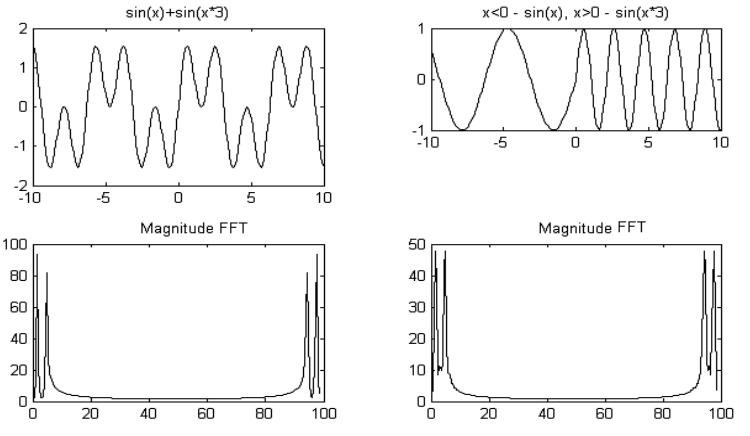
\includegraphics[scale = 0.7]{img/noninf_furie.png}}
		\end{center}
		\caption{Пример неинформативности преобразования Фурье}
		\label{ris:noninform_furie}
	\end{figure}
	
	Речевой сигнал является примером нестационaрного процессa, в котором информaтивным является сам фaкт изменения его частотно-временных харaктеристик.

	Для анализа таких процессов требуются базисные функции, способные выявлять в исследуемом сигнале как частотные, так и его временные  характеристики, то есть функции со свойствами частотно-временной локализации. Такие возможности предоставляют вейвлеты, являющиеся обобщением спектрального анализа ~\cite{magistr}.
	
	Ниже приведена общая формула вейвлет-преобразования функции $f(t)$.
	
	\begin{equation}\label{eq:wavelet-main}
		W_{\Psi}(x, a) = \frac{1}{\sqrt{a}}\int_{-\infty}^{\infty}f(t)\Psi(\frac{t-x}{a})dt,
	\end{equation}
	
	где
	\begin{itemize}
		\item $\Psi(\frac{t-x}{a})$ - вейвлет;
		\item a - масштабный коэффициент;
		\item x - параметры сдвига.
	\end{itemize}
	
	Вейвлеты – функции двух аргументов – масштаба и сдвига. В отличие от стандартного преобразования Фурье, они позволяют обрабатывать сигнал одновременно в физическом – время, координата; и частотном пространствах. 
	
	Выбор анализирующего вейвлета определяется тем, какую информацию необходимо извлечь из сигнала. Каждый вейвлет имеет характерные особенности во временном и в частотном пространстве, поэтому иногда с помощью разных вейвлетов можно полнее выявить и подчеркнуть те или иные свойства анализируемого сигнала.

	Таким образом, вейвлет-преобразование обеспечивает двумерное представление исследуемого сигнала в частотной области в плоскости частота-\linebreak положение. Аналогом частоты при этом является масштаб аргумента базисной функции (чаще всего – времени), а положение характеризуется её сдвигом. Это позволяет найти особенности сигналов, одновременно локализуя их на временной шкале. Другими словами, вейвлет-анализ можно охарактеризовать как спектральный анализ локальных возмущений.
	
	Используя вейвлет-преобразование, сигнал можно представить как последовательность образов с разной степенью детализации, что позволяет найти локальные особенности сигнала и классифицировать их по интенсивности.
	
	{\bf Многомасштабный Вейвлет-анализ} основывается на разложении сигнала по функциям, образующим ортонормированный базис. Каждую функцию можно разложить на некотором заданном уровне разрешения (масштабе) $j_n$ в ряд вида ~\cite{magistr}:
	
	\begin{equation}
		f(x) = \sum_{k=0}^{2M-1}s_{j_n,k}\varphi_{j_n,k}+\sum_{j\geq j_n}^{j_{max}}\sum_{k=0}^{2M-1}d_{j,k}\Psi_{j,k},
	\end{equation}
	
	где
	
	\begin{itemize}
		\item $\varphi_{j_n,k}$ и $\Psi_{j,k}$ - масштабированные и смещенные версии скейлинг-функции (масштабной функции) $\varphi$ и материнского вейвлета $\Psi$;
		\item $s_{j,k}$ - коэффициенты аппроксимации;
		\item $d_{j,k}$ - детализирующие коэффициенты.
	\end{itemize}

	На рисунках ~\ref{ris:wavelet_simlet} -~\ref{ris:wavelet_dobeshi4} представлены аналитические графики функций $\varphi$ и $\Psi$ указанных вейвлетов.
	
	\begin{figure}[h!]
		\begin{center}
			{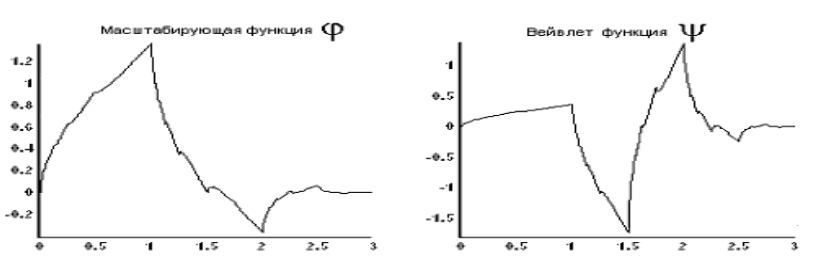
\includegraphics[scale = 0.9]{img/wavelet_simlet.png}}
		\end{center}
		\caption{Аналитические графики функций $\varphi$ и $\Psi$, вейвлет Симлета}
		\label{ris:wavelet_simlet}
	\end{figure}

	\begin{figure}[h!]
		\begin{center}
			{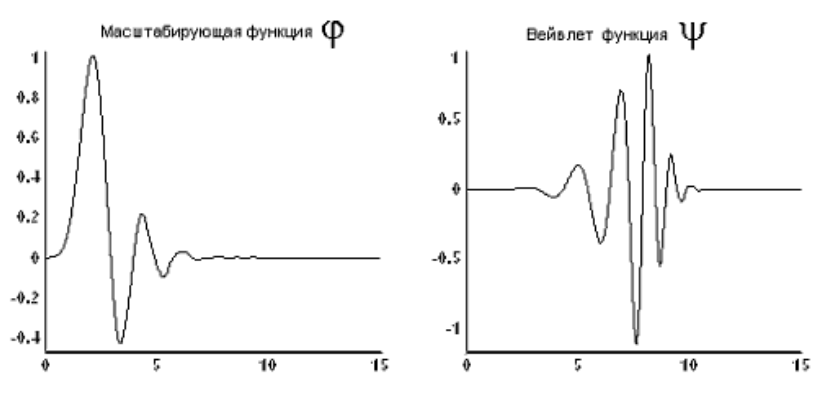
\includegraphics[scale = 0.7]{img/wavelet_dobeshi8.png}}
		\end{center}
		\caption{Аналитические графики функций $\varphi$ и $\Psi$, вейвлет Добеши 8}
		\label{ris:wavelet_dobeshi8}
	\end{figure}

	\newpage

	\begin{figure}[h!]
		\begin{center}
			{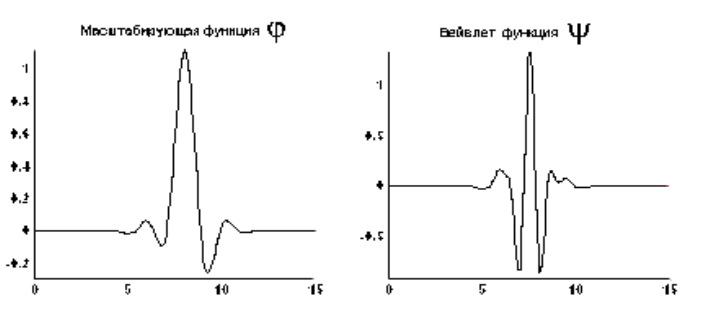
\includegraphics[scale = 1.0]{img/wavelet_simlet8.png}}
		\end{center}
		\caption{Аналитические графики функций $\varphi$ и $\Psi$, вейвлет Симлета 8}
		\label{ris:wavelet_simlet8}
	\end{figure}

	\begin{figure}[h!]
		\begin{center}
			{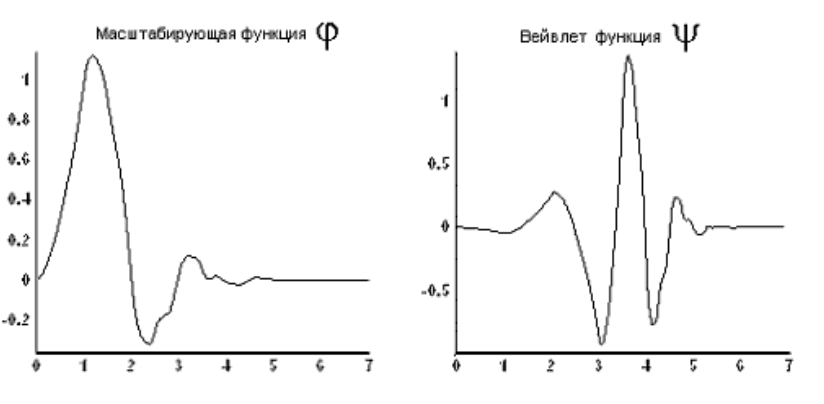
\includegraphics[scale = 0.8]{img/wavelet_dobeshi4.png}}
		\end{center}
		\caption{Аналитические графики функций $\varphi$ и $\Psi$, вейвлет Добеши 4}
		\label{ris:wavelet_dobeshi4}
	\end{figure}

	Масштабирование и смещение функций $\varphi_{j,k}$ и $\Psi_{j,k}$ находится следующим образом:
	
	\begin{equation}
		\varphi_{j,k} = 2^{j/2}\varphi(2^jx-k),
	\end{equation}

	\begin{equation}
		\Psi_{j,k} = 2^{j/2}\Psi(2^jx-k),
	\end{equation}

	В свою очередь сами функции $\varphi$ и $\Psi$ определяются следующим образом:
	
	\begin{equation}
		\varphi = \sqrt{2}\sum_{k=0}^{2M-1}h_k\varphi(2x-k),
	\end{equation}

	\begin{equation}
		\Psi = \sqrt{2}\sum_{k=0}^{2M-1}g_k\Psi(2x-k),
	\end{equation}

	где $g_k = (-1)^kh_{2M-k-1}$
	
	Таким образом, ортогональный вейвлет-анализ сводится к нахождению коэффициентов аппроксимации и детализирующих коэффициентов в разложении сигнала $f(t)$ по формуле (\ref{eq:wavelet-main}).
	
	\begin{flushleft}
		{\bf Достоинства вейвлет-преобразования:}
	\end{flushleft}
	\begin{itemize}
		\item вейвлетные преобразования обладают всеми достоинствами
		преобразований Фурье;
		\item вейвлетные базисы могут быть хорошо локализованными как по
		частоте, так и по времени. При выделении в сигналах хорошо
		локализованных разномасштабных процессов можно рассматривать только те масштабные уровни разложения, которые представляют интерес;
		\item базисные вейвлеты могут реализоваться функциями различной
		гладкости.
	\end{itemize}

	\begin{flushleft}
		{\bf Недостатки:}
	\end{flushleft}
	\begin{itemize}
		\item относительная сложность преобразования.
	\end{itemize}
	
	\subsubsection{Преобразование Гильберта-Хуанга}
	
	Под преобразованием Гильберта-Хуанга (Hilbert-Huang transform – HHT) понимается метод эмпирической модовой декомпозиции (EMD) нелинейных и нестационарных процессов и Гильбертов спектральный анализ (HSA) ~\cite{magistr}. Этот метод потенциально жизнеспособен для нелинейного и нестационарного анализа данных ~\cite{hilbert_huang}, специально для частотно-энергетических временных представлений.
	
	EMD-HSA предложил Норден Хуанг в 1995 в США (NASA) для изучения поверхностных волн тайфунов, включая возможность на анализ произвольных временных рядов коллективом соавторов в 1998 г.. В последующие годы, активно расширяя применения алгоритма для других новых отраслей науки и техники, взамен термина EMD-HSA был принят более короткий термин преобразования HHT.
	
	{\bf EMD (Empirical Mode Decomposition)} – метод разложения сигналов на функции, получившие названия внутренних или <<эмпирических мод>>. Метод представляет собой адаптивную итерационную вычислительную процедуру разложения исходных данных (непрерывных или дискретных сигналов) на эмпирические моды или внутренние колебания.
	
	{\bf Огибающие сигналов.} У каждого сигнала присутствуют локальные экстремумы: чередующиеся локальные максимумы и локальные минимумы с произвольным расположением по координатам (независимым переменным) сигналов. По этим экстремумам с использованием методов аппроксимации можно построить две огибающие сигналов: нижнюю – построенную по точкам локальных минимумов, и верхнюю – построенную по точкам локальных максимумов, а также функцию <<среднего значения огибающих>>, которой отвечает срединная линия, расположенная в точности между нижней и верхней огибающими ~\cite{magistr}.
	
	Модовая декомпозиция сигналов основана на предположении, что любые данные состоят из различных внутренних колебаний IMF. В любой момент времени данные могут иметь множество сосуществующих внутренних колебаний – IMFs. Каждое колебание, линейное или нелинейное, представляет собой модовую функцию, которая имеет экстремумы и нулевые пересечения. Кроме того, колебания в определенной степени <<симметричны>> относительно локального среднего значения. Конечные сложные данные образуются суммой модовых функций, наложенных на региональный тренд сигнала.
	
	Эмпирическая мода – это такая функция, которая обладает следующими свойствами:
	\begin{enumerate}
		\item количество экстремумов функции (максимумов и минимумов) и количество пересечений нуля не должны отличаться более чем на единицу;
		\item в любой точке функции среднее значение огибающих, определенных локальными максимумами и локальными минимумами, должно быть нулевым.
	\end{enumerate}

	IMF представляет собой колебательный режим, но вместо постоянной амплитуды и частоты, как в простой гармонике, у IMF могут быть переменная амплитуда и частота, как функции независимой переменной. Первое свойство гарантирует, что локальные максимумы функции всегда положительны, локальные минимумы соответственно отрицательны, а между ними всегда имеют место пересечения нулевой линии. Второе свойство гарантирует, что мгновенные частоты функции не будут иметь нежелательных флуктуаций, являющихся результатом асимметричной формы волны.
	
	Любую функцию и любой произвольный сигнал, изначально содержащие произвольную последовательность локальных экстремумов (минимум 2), можно разделить на семейство функций IMFs и остаточный тренд. Если данные лишены экстремумов, но содержат точки перегиба (<<скрытые>> экстремумы наложения модовых функций и крутых трендов), то для открытия экстремумов может использоваться дифференцирование сигнала.
	
	Схема преобразования Гильберта-Хуанга делится на две части. На первом этапе, экспериментальные данные разлагаются в ряд внутренних модовых функций (IMFs). Эта декомпозиция рассматривается как расширение данных в терминах внутренних модовых функций. Иначе, эти внутренние модовые функции представлены как базис преобразования, которое может быть линейным или нелинейным, как диктуется по условиям. Так как IMFs имеют хорошие Гильбертовы преобразования, то могут быть вычислены соответствующие мгновенные частоты. На следующем этапе локализуются любые явления, как во времени, так и на частотной оси. Локальная энергия и мгновенная частота, выведенная из IMFs, дают дистрибутивные <<энергетические время-частотные>> данные, и такое представление, определяемое как Гильбертов спектр: 
	
	\begin{equation}
		r_j(t) = r_{j-1}-c_j(t)
	\end{equation}

	Пусть имеется произвольный сигнал $y(t)$. Сущность метода EMD заключается в последовательном вычислении функций эмпирических
	мод $c(t)$ и остатков $r_j(t) = r_{j-1}-c_j(t)$, где $j=1,2,3,..,n$ при $r_0=y(t)$. Результатом разложения будет представление сигнала в виде суммы модовых функций и конечного остатка:
	
	\begin{equation}\label{eq:huang_main}
		x(t) = \sum_{j=1}^{n}c_j(t)+r_n(t),
	\end{equation}

	где n - количество эмпирических мод, которое устанавливается в ходе вычислений.
	
	Алгоритм эмпирической декомпозиции сигнала складывается из следующих операций преобразования:
	
	\begin{enumerate}
		\item находится в сигнале $y(k)$ положение всех локальных экстремумов, максимумов и минимумов процесса (номера точек $k_{i.ext}$ экстремумов), и значения в этих точках (рисунок \ref{ris:huang_local_extr}). Между этими экстремумами сосредоточена вся информация сигнала. Группируются массивы координат $k_{i.ext}$ для максимумов и минимумов, и соответствующих им амплитудных значений $y(k_{i.ext})$. Число строк в массивах максимумов и минимумов не должно отличаться более чем на 1.
		
		\begin{figure}[h!]
			\begin{center}
				{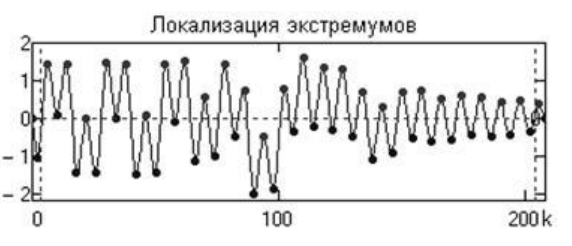
\includegraphics[scale = 0.9]{img/huang_local_extr.png}}
			\end{center}
			\caption{Локализация экстремумов в сигнале}
			\label{ris:huang_local_extr}
		\end{figure}
		
		\item Применяя сплайны вычисляются верхняя $u_t(k)$ и нижняя $u_b(k)$ огибающие процесса соответственно, по максимумам и минимумам, как это показано на рисунке \ref{ris:huang_interp_extr}. Определяется функция средних значений $m_1(k)$ между огибающими (рисунок \ref{ris:huang_interp_extr}).
		
		\begin{figure}[h!]
			\begin{center}
				{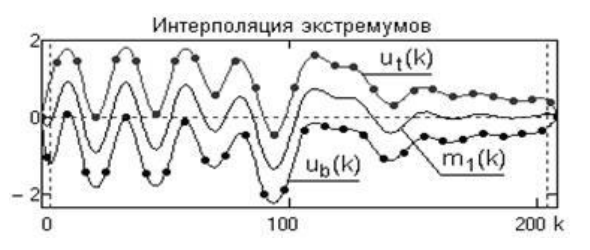
\includegraphics[scale = 0.9]{img/huang_interp_extr.png}}
			\end{center}
			\caption{Интерполяция экстремумов и построение огибающих}
			\label{ris:huang_interp_extr}
		\end{figure}
	
		Далее, определяется функция средних значений $m_1(k)$ между огибающими.
		
		\begin{equation}
			m_1(k) = \frac{u_t(k)+u_b(k)}{2},
		\end{equation}
	
		\newpage
	
		Разность между сигналом $y(k)$ и функцией $m_1(k)$ дает первую компоненту отсеивания - функцию $h_1(k)$, которая является первым приближением к первой функции IMF:
		
		\begin{equation}
			h_1(k) = y(k)-m_1(k),
		\end{equation}
	
		\item Повторяются операции 1) и 2), принимая вместо $y(k)$ функцию $h_1(k)$, и находятся второе приближение к первой функции IMF – функцию $h_2(k)$.
		
		\begin{equation}
			h_2(k) = h_1(k)-m_2(k),
		\end{equation}
	
		Последующие итерации выполняются аналогичным образом:
		
		\begin{equation}\label{eq:huang_iters}
			h_i(k) = h_{i-1}(k)-m_i(k),
		\end{equation}
	
		По мере увеличения количества итераций функция $m_i(k)$ стремится к нулевому значению, а функция $h_i(k)$ – к неизменяемой форме.
		
		Последнее значение $h_i(k)$ итераций принимается за наиболее высокочастотную функцию $r_1(k) = y(k)-c_1(k)$ семейства IMF, которая непосредственно входит в состав исходного сигнала $y(k)$. Это позволяет вычесть $c_1(k)$ из состава сигнала и оставить в нем более низкочастотные составляющие $r_1(k) = y(k)-c_1(k),$
		
		На рисунке \ref{ris:huang_find_low_parts} показано графическое представление вычитания из сигнала высокочастотной составляющей, сформированной по алгоритму, заданному (\ref{eq:huang_main})-(\ref{eq:huang_iters}).
		
		\begin{figure}[h!]
			\begin{center}
				{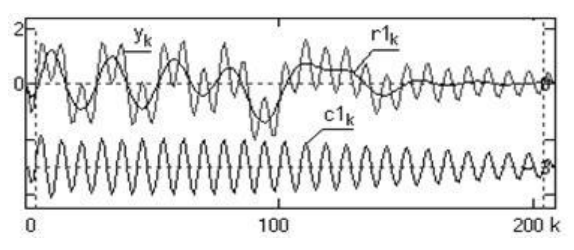
\includegraphics[scale = 1.1]{img/huang_find_low_parts.png}}
			\end{center}
			\caption{Выявление низкочастотных составляющих в сигнале}
			\label{ris:huang_find_low_parts}
		\end{figure}
	
		Следующая внутренняя модовая функция находится, повторяя операции 1)-3) декомпозиции, описанные выше, с той разницей, что входным сигналом является остаток $r_1(k)$.
		
		Шаги 1)-3) повторяются для всех последующих $r_j(k)$, и результат будет представлять последовательность вычислений:
		
		\begin{equation}
			r_1(k)-c_2(k)=r_2(k),...,r_{n-1}(k)-c_n(k)=r_n(k),
		\end{equation}
	
		Метод EMD закончен, когда остаток, в идеале, не содержит экстремумов. Это означает, что остаток – или константа или монотонная функция. Извлечённые IMFs симметричны, имеют уникальные локальные частоты, различные IMFs не показывают ту же самую частоту в то же самое время. Другими словами, остановка декомпозиции сигнала должна происходить при максимальном <<выпрямлении>> остатка, то есть превращения его в тренд сигнала по интервалу задания с числом экстремумов не более 2-3 ~\cite{magistr}.
		
	\end{enumerate}

	\begin{flushleft}
		{\bf Достоинства преобразования Гильберта-Хуанга:}
	\end{flushleft}
	\begin{itemize}
		\item базис, используемый при разложении (набор эмпирических мод) конструируется непосредственно из того сигнала, с которым ведется работа, что позволяет учесть все его локальные особенности, внутреннюю структуру, наличие нежелательных особенностей (шумы, тренды, аномальные выбросы, пропущенные значения).
	\end{itemize}
	
	\begin{flushleft}
		{\bf Недостатки:}
	\end{flushleft}
	\begin{itemize}
		\item гораздо более высокая вычислительная сложность по сравнению с вейвлет-преобразованием.
	\end{itemize}
	
	\subsection{Алгоритмы классификации}
	
	После получения акустических характеристик сигнала на заданных интервалах времени необходимо определить границы между основными лингвистическими элементами языка.
	
	Большинство работ, связанных с автоматической сегментацией речевого сигнала, для решения данной задачи используют определенные закономерности, эвристики в изменении значений выделенных признаков речевого сигнала в момент межфонемного перехода \cite{disertation}. Эти закономерности чаще всего не имеют большой теоретической базы и лишь основываются на экспериментальном опыте других работ.
	
	Так, в работах \cite{vevlet_1}, \cite{vevlet_2} сегментация речевого сигнала на фрагменты, осуществляющая на базе Вейвлет-преобразования, используют тот факт, что на межфонемных переходах сигнал претерпевает значительные изменения сразу на многих масштабах исследования и, соответственно, характеризуется возрастанием вейвлет-коэффициентов для многих уровней детализации, в то время как на стационарных участках фонем вейвлет-коэффициенты оказываются сгруппированными вблизи определённых масштабов. Таким образом, отыскание межфонемных границ сводится к отысканию моментов увеличения вейвлет-коэффициентов на значительном количестве уровней масштабирования.
	
	На основе этих закономерностей формируется критерий определения межфонемных переходов, который в свою очередь также определяется экспериментальным путем, в виду чего не гарантируют, полученной в результате экспериментов точности на других данных из-за сложной структуры звукового сигнала.
	
	Исходя из приведенных выше рассуждений в данной работе решено применить метод классификации машинного обучения.
	
	\subsubsection{Формальная постановка задачи классификации}\label{formal_classification}
	
	Пусть $X$ — множество описаний объектов,
	
	$Y$ - конечное множество меток классов. 
	
	Существует неизвестная целевая зависимость — отображение $y^{*}:\; X\to Y$, значения которой известны только на объектах конечной обучающей выборки $X^m = \{(x_1,y_1),\dots,(x_m,y_m)\}$. 
	
	Требуется построить алгоритм $a: X\to Y$, способный классифицировать произвольный объект $x \in X$.
	
	Для решения этой задачи могут быть использованы следующие методы классификации \cite{classification_methods}:
	
	\begin{itemize}
		\item вероятностные (<<наивный>> Байес);
		\item метрические (метод k ближайших соседей);
		\item логические (решающее дерево);
		\item линейные (метод опорных векторов, логистическая регрессия);
		\item методы на основе искусственных нейронных сетей (FFBP, RNN, CNN).
	\end{itemize}
	
	Рассмотрим наиболее популярные подходы для каждого из методов.
	
	\subsubsection{Наивный байесовский классификатор}
	
	{\bf Метод Байеса (Naive Bayes, NB)} относится к вероятностным методам классификации.
	
	Пусть $P(c_i|d)$ - вероятность того, что объект, представленный вектором $d = (t_1, ..., t_n)$, соответствует категории $c_j$ для $i = 1, ...|C|$. Задача классификатора заключается в том, чтобы подобрать такие значения $c_i$ и $d$, при которых значение вероятности $P(c_i|d)$ будет максимальным:
	
	\begin{equation}
		CSV(d) = \underset{c_i\in C}{argmax} P(c_i|d)
	\end{equation}

	Для вычисления значений $P(c_i|d)$ используется теорема Байеса:
	
	\begin{equation}
		P(c_i|d) = \frac{P(c_i) P(d|c_i)}{P(d)},
	\end{equation}\label{eq:bayes}

	где
	
	\begin{itemize}
		\item $P(c_i)$ - априорная вероятность того, что вектор $d$ отнесен к категории $c_i$;
		\item $P(d|c_i)$ - вероятность найти вектор $d = (t_1, ..., t_n)$ в категории $c_i$;
		\item $P(d)$ - вероятность того, что произвольно взятый объект можно представить в виде вектора признаков $d = (t_1, ..., t_n)$.
	\end{itemize}

	$P(d)$ не зависит от категории $c_i$, а значения $t_1, ..., t_n$ заданы заранее, поэтому знаменатель не влияет на выбор наибольшего из значений $P(c_i|d)$.
	
	Вычисление $P(d|c_i)$ затруднительно из-за большого количества признаков $t_1, ..., t_n$ поэтому делают <<наивное>> предположение о том, что любые случайные величины не зависят друг от друга.
	
	Исходя из этого допущения можно воспользоваться формулой:
	
	\begin{equation}
		P(d|c_i) = \prod_{k=1}^{n} P(t_k|c_i)
	\end{equation}

	\begin{flushleft}
		{\bf Преимущества метода:}
	\end{flushleft}
	
	\begin{itemize}
		\item высокая скорость работы;
		\item поддержка инкрементного обучения;
		\item относительно простая реализация программная реализация алгоритма;
		\item легкая интерпретируемость результатов алгоритма.
	\end{itemize}

	\begin{flushleft}
		{\bf Недостатки метода:}
	\end{flushleft}

	\begin{itemize}
		\item относительно низкое качество классификации по сравнению с другими методами;
		\item неспособность учитывать зависимость результата классификации от сочетания признаков из-за допущения о их независимости друг от друга.
	\end{itemize}
		
	\subsubsection{Метод k-ближайших соседей}
	
	{\bf Метод $k$ ближайших соседей (k Nearest Neighbours, KNN)} относится к метрическим методам классификации. 
	
	Чтобы найти категорию, соответствующую объекту $d$, классификатор сравнивает $d$ со всеми объектами из обучающей выборки $L$, то есть для каждого $d_z \in L$ вычисляется расстояние $ρ(d_z, d)$. Далее из обучающей выборки выбираются $k$ объектов, ближайших к $d$. Согласно методу $k$ ближайших соседей, объект $d$ считается принадлежащим тому классу, который является наиболее распространненным среди соседей данного объекта, то есть для каждого класса $c_i$ вычисляется функция ранжирования:
	
	\begin{equation}
		CSV(d) = \sum_{d_z\in L_k(d)} p(d_z, d) * \Upphi(d_z, c_i),
	\end{equation}

	где
	
	\begin{itemize}
		\item $L_k(d)$ - ближайшие $k$ объектов из $L$ к $d$;
		\item $\Upphi(d_z, c_i)$ - количество объектов $d_z$ обучающей выборки относящиеся к категории $c_i$.
	\end{itemize}

	\begin{flushleft}
		{\bf Преимущества метода:}
	\end{flushleft}

	\begin{itemize}
		\item возможность обновления обучающей выборки без переобучения классификатора; 
		\item устойчивость алгоритма к аномальным выбросам в исходных данных; 
		\item относительно простая программная реализация алгоритма;
		\item легкая интерпретируемость результатов работы алгоритма;
		\item хорошее обучение в случае с линейно неразделимыми выборками.
	\end{itemize}
	
	\begin{flushleft}
		{\bf Недостатки метода:}
	\end{flushleft}

	\begin{itemize}
		\item репрезентативность набора данных, используемого для алгоритма;
		\item высокая зависимость результатов классификации от выбранной метрики;
		\item большая длительность работы из-за необходимости полного  перебора обучающей выборки; 
		\item невозможность решения задач большой размерности по количеству классов и объектов. 
	\end{itemize}
	
	\subsubsection{Метод деревьев решений (Decision Trees, DT)}
	
	{\bf Метод деревьев решений (Decision Trees, DT)} относится к логическим методам классификации. 
	
	Деревом решений называют ациклический граф, по которому производится классификация объектов, описанных набором признаков. Каждый узел дерева содержит условие ветвления по одному из признаков.  У каждого узла столько ветвлений, сколько значений имеет выбранный  признак. В процессе классификации осуществляются последовательные переходы от одного узла к другому в соответствии со значениями  признаков объекта. 
	
	Классификация считается завершенной, когда достигнут один из листьев (конечных  узлов) дерева. Значение этого листа  определит класс, которому принадлежит рассматриваемый объект. На  практике обычно используют бинарные деревья решений, в которых принятие решения перехода по ребрам осуществляется простой  проверкой наличия признака в объекте. Если значение признака меньше определенного значения, выбирается одна ветвь, если больше или равно, другая.
	
	\begin{figure}[h!]
		\begin{center}
			{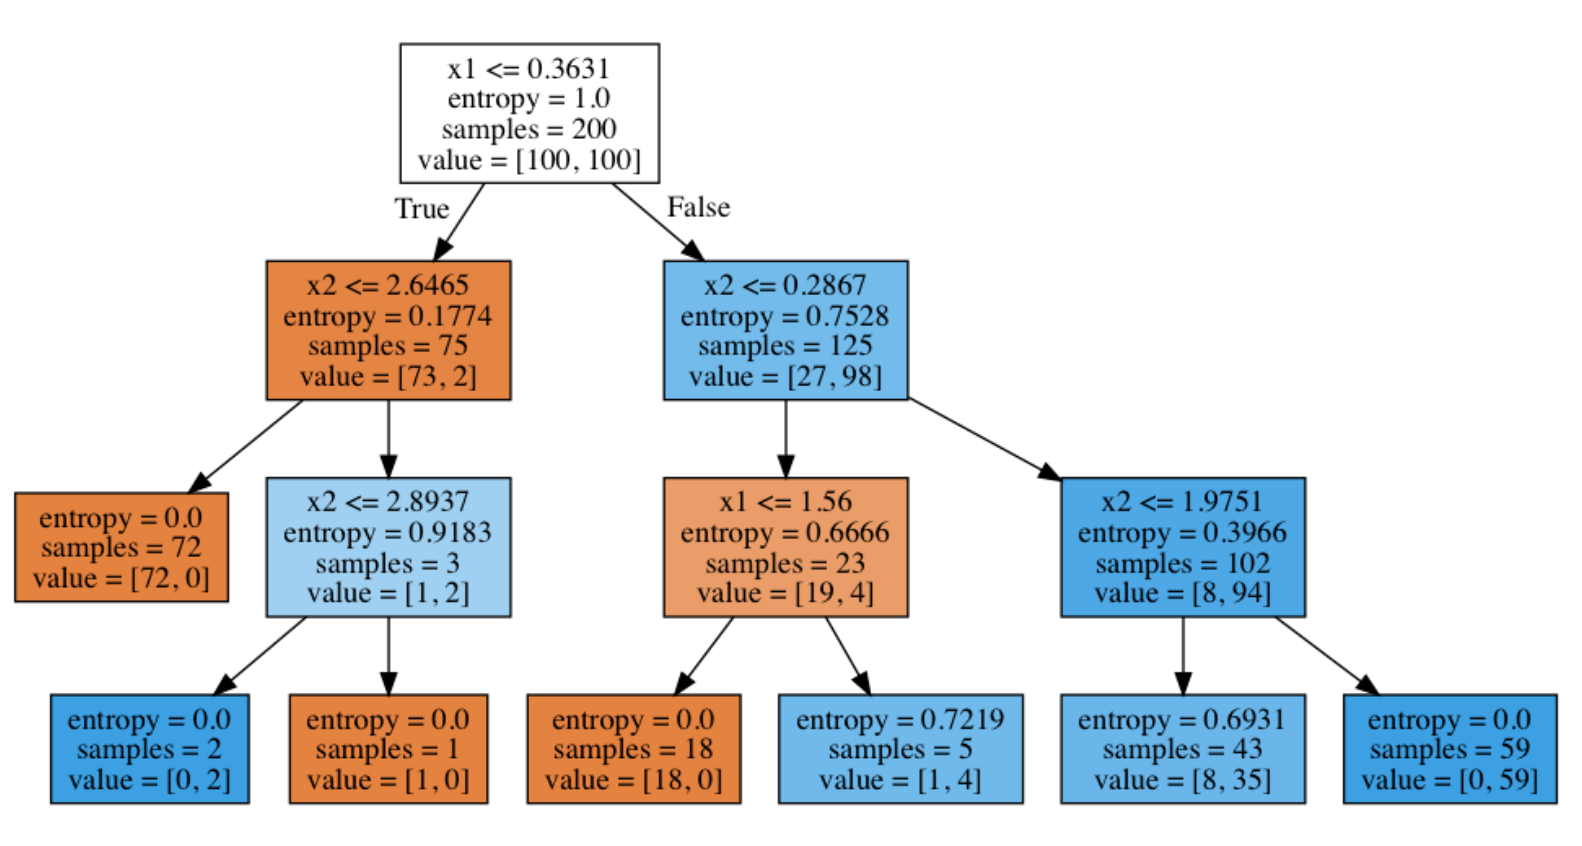
\includegraphics[scale = 0.45]{img/tree.png}}
		\end{center}
		\caption{Пример построенного бинарного дерева решений по двум признакам}
		\label{ris:tree}
	\end{figure}

	\begin{flushleft}
		{\bf Преимущества метода:}
	\end{flushleft}

	\begin{itemize}
		\item относительно простая программная реализация алгоритма;
		\item легкая интерпретируемость результатов работы алгоритма.
	\end{itemize}

	\begin{flushleft}
		{\bf Недостатки метода:}
	\end{flushleft}

	\begin{itemize}
		\item неустойчивость алгоритма к выбросам исходных данных;
		\item требуется большой объем данных для получения точных результатов.
	\end{itemize}
	
	\subsubsection{Метод опорных векторов}
	
	{\bf Метод опорных векторов (Support Vector Machine, SVM)} является линейным методом классификации. Рассмотрим множество объектов, которые \linebreak необходимо классифицировать. Сопоставим ему множество точек в пространстве размерности |D|.
	
	Выборку точек называют линейно разделимой, если принадлежащие разным классам точки можно разделить с помощью гиперплоскости (в двумерном случае - прямой). Необходимо провести прямую так, чтобы по одну сторону от нее лежали все точки одного класса, а по другую - все точки другого класса. Тогда для классификации неизвестных точек достаточно будет посмотреть, с какой стороны прямой они окажутся.
	
	В методе опорных векторов расстоянием между прямой и множеством точек считается расстояние между прямой и ближайшей к ней точкой из множества. Именно такое расстояние и максимизируется в данном методе. Гиперплоскость, максимизирующая расстояние до двух параллельных гиперплоскостей, называется разделяющей (на рисунке ~\ref{ris:svm} обозначена буквой L). Ближайшие к параллельным гиперплоскостям точки называются опорными векторами, через них проходят пунктирные линии.
	
	\newpage
	
	\begin{figure}[h!]
		\begin{center}
			{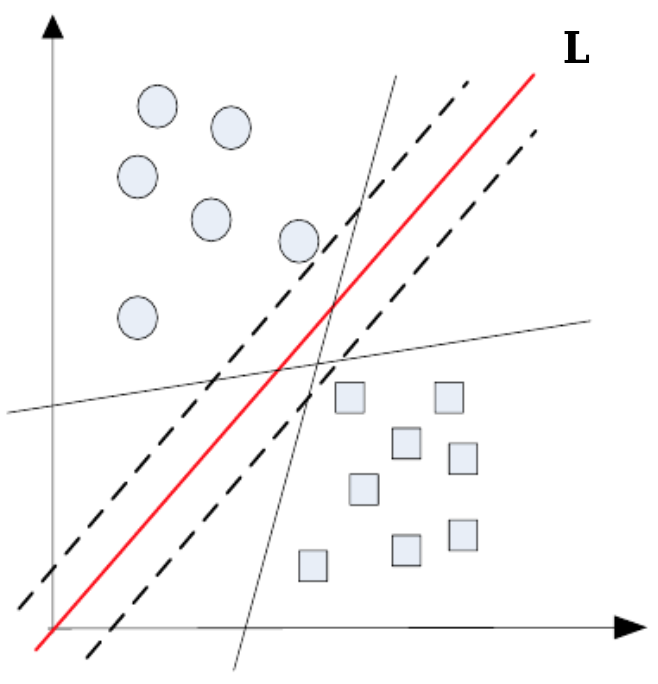
\includegraphics[scale = 0.6]{img/svm.png}}
		\end{center}
		\caption{Разделяющая гиперплоскость в методе опорных векторов}
		\label{ris:svm}
	\end{figure}

	\begin{flushleft}
		{\bf Преимущества метода:}
	\end{flushleft}

	\begin{itemize}
		\item один из наиболее качественных методов;
		\item возможность работы с небольшим набором данных для обучения;
		\item сводимость к задаче выпуклой оптимизации, имеющей единственное решение.
	\end{itemize}

	\begin{flushleft}
		{\bf Недостатки метода:}
	\end{flushleft}

	\begin{itemize}
		\item сложная интерпретируемость параметров алгоритма;
		\item неустойчивость к выбросам в исходных данных.
	\end{itemize}

	
	\subsubsection{Методы на основе искусственных нейронных сетей}
	
	Нейронная сеть — это система соединённых и взаимодействующих между собой простых процессоров (нейронов), соединенных между собой синапсами.
	
	Существует большое количество разновидностей нейронных сетей, основные из них – сети прямого распространения, рекуррентные сети,  радиально-базисные функции и самоорганизующиеся карты.
	
	Рассмотрим структуру классической нейронной сети прямого распространения (Feed Forward Back Propagation, FFBP).
	
	В нейронных сетях прямого распространения присутствуют входной слой, выходной слой и промежуточные (скрытые) слои: сигнал идет последовательно от входного слоя нейронов по промежуточным слоям к выходному. 
	
	\begin{figure}[h!]
		\begin{center}
			{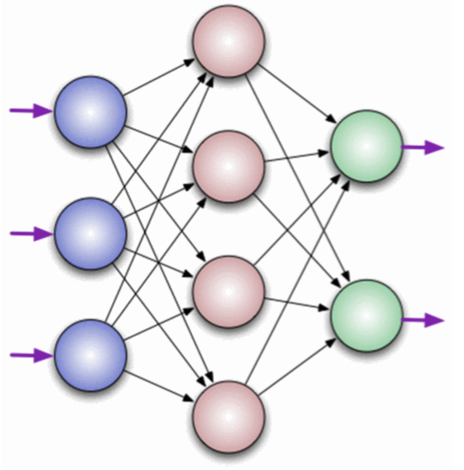
\includegraphics[scale = 0.6]{img/nn.png}}
		\end{center}
		\caption{Пример нейронных слоев (синий - входной, красный - скрытый, зеленый - выходной)}
		\label{ris:nn}
	\end{figure}

	Для классификации объекта $d_i$ при помощи нейронной сети прямого распространения веса признаков документа подаются на соответствующие входы сети. Активация распространяется по сети; значения, получившиеся на выходах, есть результат классификации. Стандартный метод обучения такой сети - метод обратного распространения ошибки.
	
	\begin{flushleft}
		{\bf Преимущества метода:}
	\end{flushleft}
	
	\begin{itemize}
		\item имеет очень высокое качество алгоритма при удачном подборе параметров;
		\item является универсальным аппроксиматором непрерывных функций;
		\item поддерживает инкрементное обучение.
	\end{itemize}
	
	\begin{flushleft}
		{\bf Недостатки метода:}
	\end{flushleft}
	
	\begin{itemize}
		\item вероятность возможной расходимости или медленной сходимости, поскольку для настройки сети используются градиентные методы;
		\item необходимость очень большого объема данных для обучения, чтобы достичь высокой точности;
		\item низкая скорость обучения;
		\item сложная интерпретируемость параметров алгоритма.
	\end{itemize}
	
	\subsection{Постановка задачи}
	
	В результате проведения анализа предметной области, существующих методов выделения признаков речевого сигнала и алгоритмов классификации, постановка задачи, которую необходимо решить в рамках данной работы, может быть определена следющим образом.
	
	Требуется спроектировать метод выделения звуков естественного языка в звучащей речи, а также разработать программный модуль для проверки работоспособности метода.
	
	\begin{figure}[h!]
		\begin{center}
			{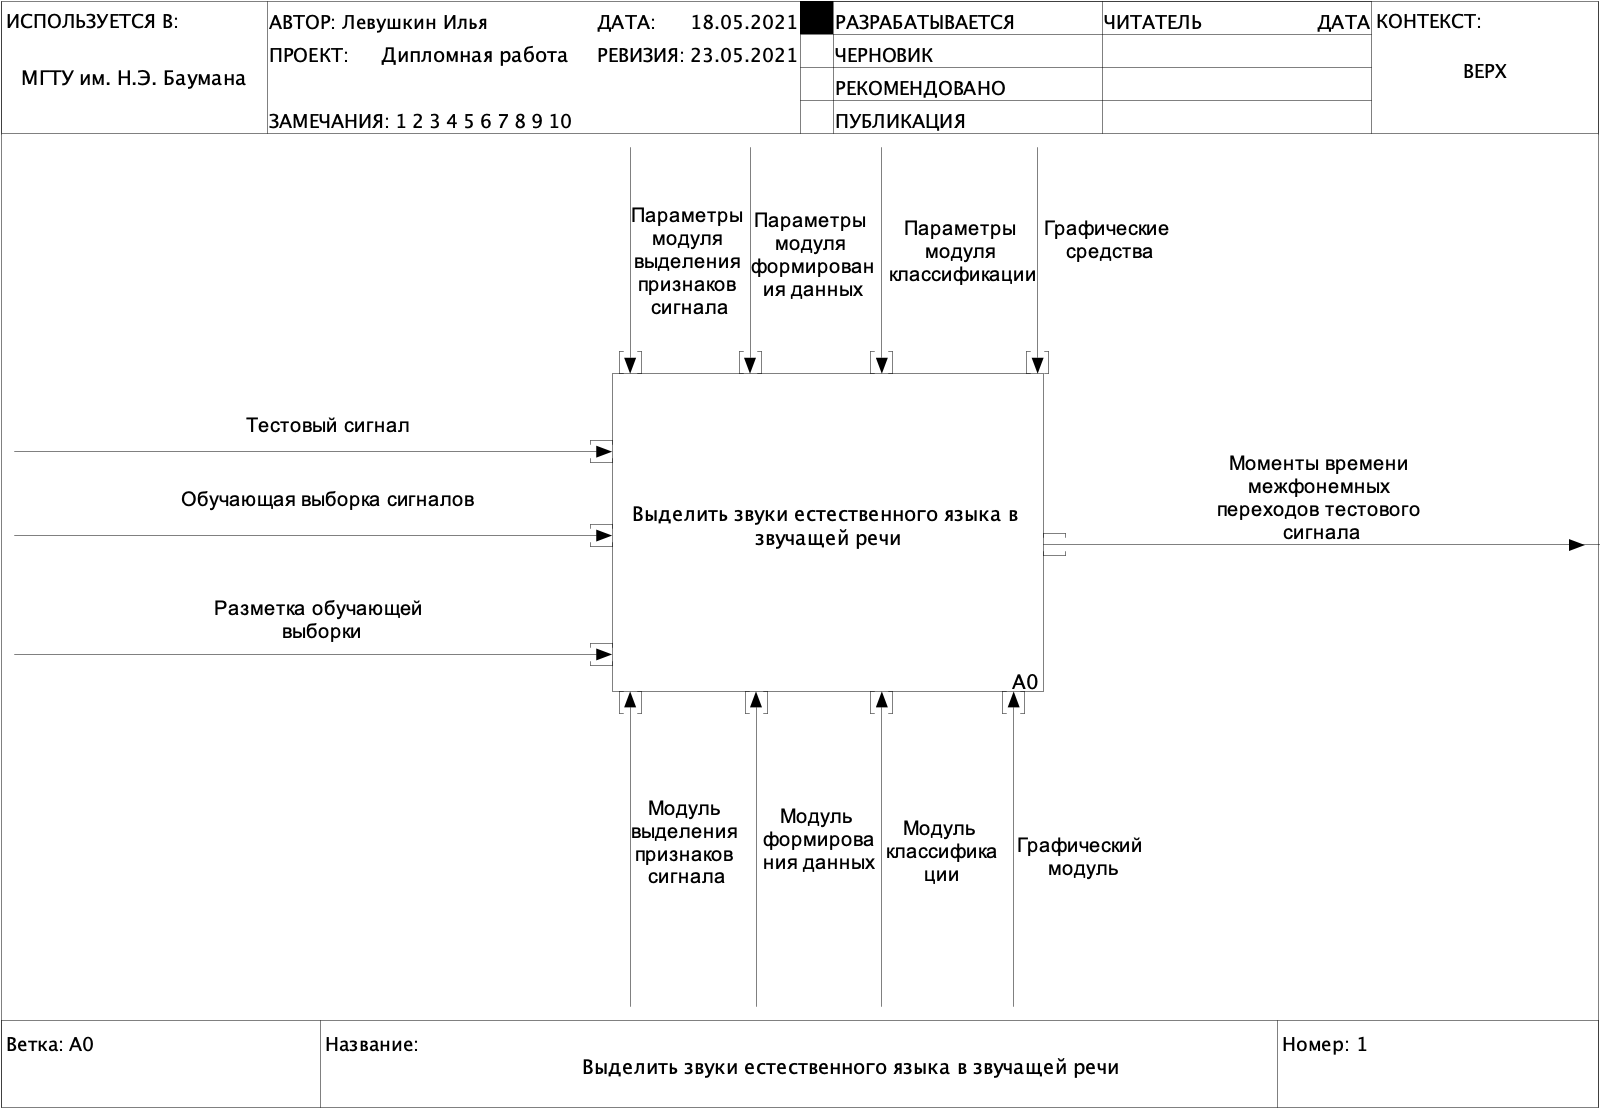
\includegraphics[scale = 0.3]{img/ramus_A0.png}}
		\end{center}
		\caption{IDEF0 диаграмма разрабатываемого модуля.}
		\label{ris:ramus_A0}
	\end{figure}
	
	{\bf Входными данными} являются аудиофайл и обучающая выборка аудиофайлов формата mp3, содержащие в себе информацию об амплитуде и частоте звуков в дискретные моменты времени, а также разметка обучающей выборки аудиофайлов в csv формате.
	
	{\bf Выходным параметром} является список моментов времени, на которых сигнал содержит межфонемные переходы.
	
	Спроектированный метод должен обеспечить возможность
	\begin{itemize}
		\item выбрать тестовый аудиофайл;
		\item вычислить список моментов времени, на которых сигнал содержит межфонемные переходы и визуализировать их графически на осциллограмме (амплитудно-временном графике сигнала) \cite{oszilograph}.
	\end{itemize}
	
	\subsection{Выводы}\label{anal_summary}
	
	В ходе анализа предметной области были описаны основные этапы распознавания речевого сигнала, а также было дано обоснование актуальности задачи сегментации речевого сигнала.
	
	Был проведен анализ существующих решений сегментации речевого сигнала на фрагменты, на основе которых были выделены два основных этапа в задаче сегментации:
	
	\begin{itemize}
		\item выделение признаков сигнала;
		\item определение межфонемных переходов на основе выделенных признаков сигнала.
	\end{itemize}

	Был произведен анализ существующих методов выделения признаков речевого сигнала. Ниже приведена сводная таблица особенностей каждого из рассмотренных методов относительно друг друга.
	
	\begin{center}
		\begin{longtable}[h!]{|p{0.12\linewidth}|p{0.16\linewidth}|p{0.13\linewidth}|p{0.1\linewidth}|p{0.16\linewidth}|p{0.16\linewidth}|}
			\hline
			{Метод} & {Базис} & {Представ-
				
				ление} & {Нелиней-
				
				ность} & {Нестационар-
				
				ность} & {Вычис-
				
				лительная сложность}\\
			\hline
			{Фурье} & {Априорный} & {Энергия-частота} & {Нет} & {Нет} & {Низкая}\\
			\hline
			{Вейвлет} & {Априорный} & {Энергия-время-частота} & {Нет} & {Да} & {Средняя}\\
			\hline
			{Гильберт-Хуанг} & {Адаптивный} & {Энергия-время-частота} & {Да} & {Да} & {Высокая}\\
			\hline
			\caption{Сравнение существующих методов выделения признаков речевого сигнала.}
		\end{longtable}
	\end{center}
	
	В данной работе было решено использовать метод, основанный на Вейвлет преобразовании, а именно, многомасштабный Вейвлет-анализ, поскольку он учитывает нестационарность человеческой речи, а также имеет относительно невысокую вычислительную сложность по сравнению с преобразованием Гильберта-Хуанга, что имеет большое значение в системах распознавания речи.
	
	Также, было обнаружено, что большинство работ используют закономерности, эвристики, основанные на экспериментальном опыте других работ и не имеющие под собой существенной теоретической базы, в виду чего эти решения не гарантируют, полученной в результате экспериментов, точности на других данных.
	
	Поэтому, в качестве альтернативы было решено использовать наиболее оптимальный для задачи определения межфонемных интервалов сигнала алгоритм классификации на основе выделенных признаков сигнала.
	
	Ниже приведена сводная таблица наиболее важных особенностей для решения поставленной задачи каждого из методов классификации относительно друг друга для малого объема обучающей выборки.
	
	\begin{center}
		\begin{longtable}[h!]{|p{0.23\linewidth}|p{0.15\linewidth}|p{0.23\linewidth}|p{0.23\linewidth}|}
			\hline
			{Метод} & {Качество обучения} & {Скорость работы} & {Поддержка 
				
				инкрементного
			
		обучения}\\
			\hline
			{Наивный Байес} & {Низкое} & {Высокая} & {Есть}\\
			\hline
			{k-ближайших соседей (KNN)} & {Среднее} & {Низкая} & {Есть}\\
			\hline
			{Деревья решений (DT)} & {Среднее} & {Средняя} & {Нет}\\
			\hline
			{Опорные вектора (SVM)} & {Высокое} & {Средняя} & {Нет}\\
			\hline
			{Искусственные нейронные сети} & {Среднее} & {Низкая} & {Есть}\\
			\hline
			\caption{Сравнение существующих методов классификации объектов.}
		\end{longtable}
	\end{center}
	
	
	В данной работе было решено использовать метод опорных векторов из-за недостаточно большого объема обучающей выборки. Метод SVM дает наилучшее качество обучения на небольшом наборе данных, а также не требует значительных ресурсных затрат для обучения и предсказания результатов по сравнению с другими методами.
	
	\pagebreak
	
	\section{Конструкторская часть}\label{constructor}
	
	Данный раздел содержит в себе следующие задачи:
	\begin{itemize}
		\item изложение принципов спроектированного метода выделения звуков естественного языка в звучащей речи;
		\item подробное описание всех этапов разработанного алгоритма, реализующего данный метод;
		\item проектирование архитектуры системы, проверяющей работоспособность данного метода.
		\item описание формата входных и выходных данных и структуры ПО;
	\end{itemize}
	
	\subsection{Метод выделения звуков естественного языка в звучащей речи}
	
	Данный метод состоит из двух основных этапов:
	
	\begin{itemize}
		\item формирования признаков из поступающего на вход речевого сигнала одним из существующих методов выделения признаков сигнала;
		\item получения границ межфонемных переходов из сформированных признаков сигнала при помощи применения алгоритмов классификации.
	\end{itemize}

	На вход данный метод получает цифровой сигнал, содержащий в себе значения амплитуд (уровней сигнала) в дискретные моменты времени, а на выходе выдает список границ (моментов времени в секундах) межфонемных переходов (переходов с одного лингвистического элемента языка ~\cite{ling_elem} к другому) естественного языка в звучащей речи.
	
	\subsection{Описание алгоритма метода выделения звуков естественного \linebreak языка в звучащей речи}
	
	Алгоритм, реализующий данный метод, состоит из следующих этапов:
	
	\begin{enumerate}
		\item выделение признаков речевых сигналов из проверяемого сигнала и обучающей выборки (рисунок \ref{ris:ramus_A1-A5} блок A1);
		\item формирование данных для применения на них (обучения и предсказания результатов) модели классификации (рисунок \ref{ris:ramus_A1-A5} блок A2);
		\item обучение модели классификации на сформированной обучающей выборке (рисунок \ref{ris:ramus_A1-A5} блок A3);
		\item применение модели классификации на тестовых данных (проверяемом сигнале) для получения предсказанных значений - межфонемных переходов (рисунок \ref{ris:ramus_A1-A5} блок A4);
		\item графическое представление результатов предсказания (рисунок \ref{ris:ramus_A1-A5} блок A5).
	\end{enumerate}
	
	Ниже приведена IDEF0-диаграмма иллюстрирующая основные этапы алгоритма.
	
	\begin{figure}[h!]
		\begin{center}
			{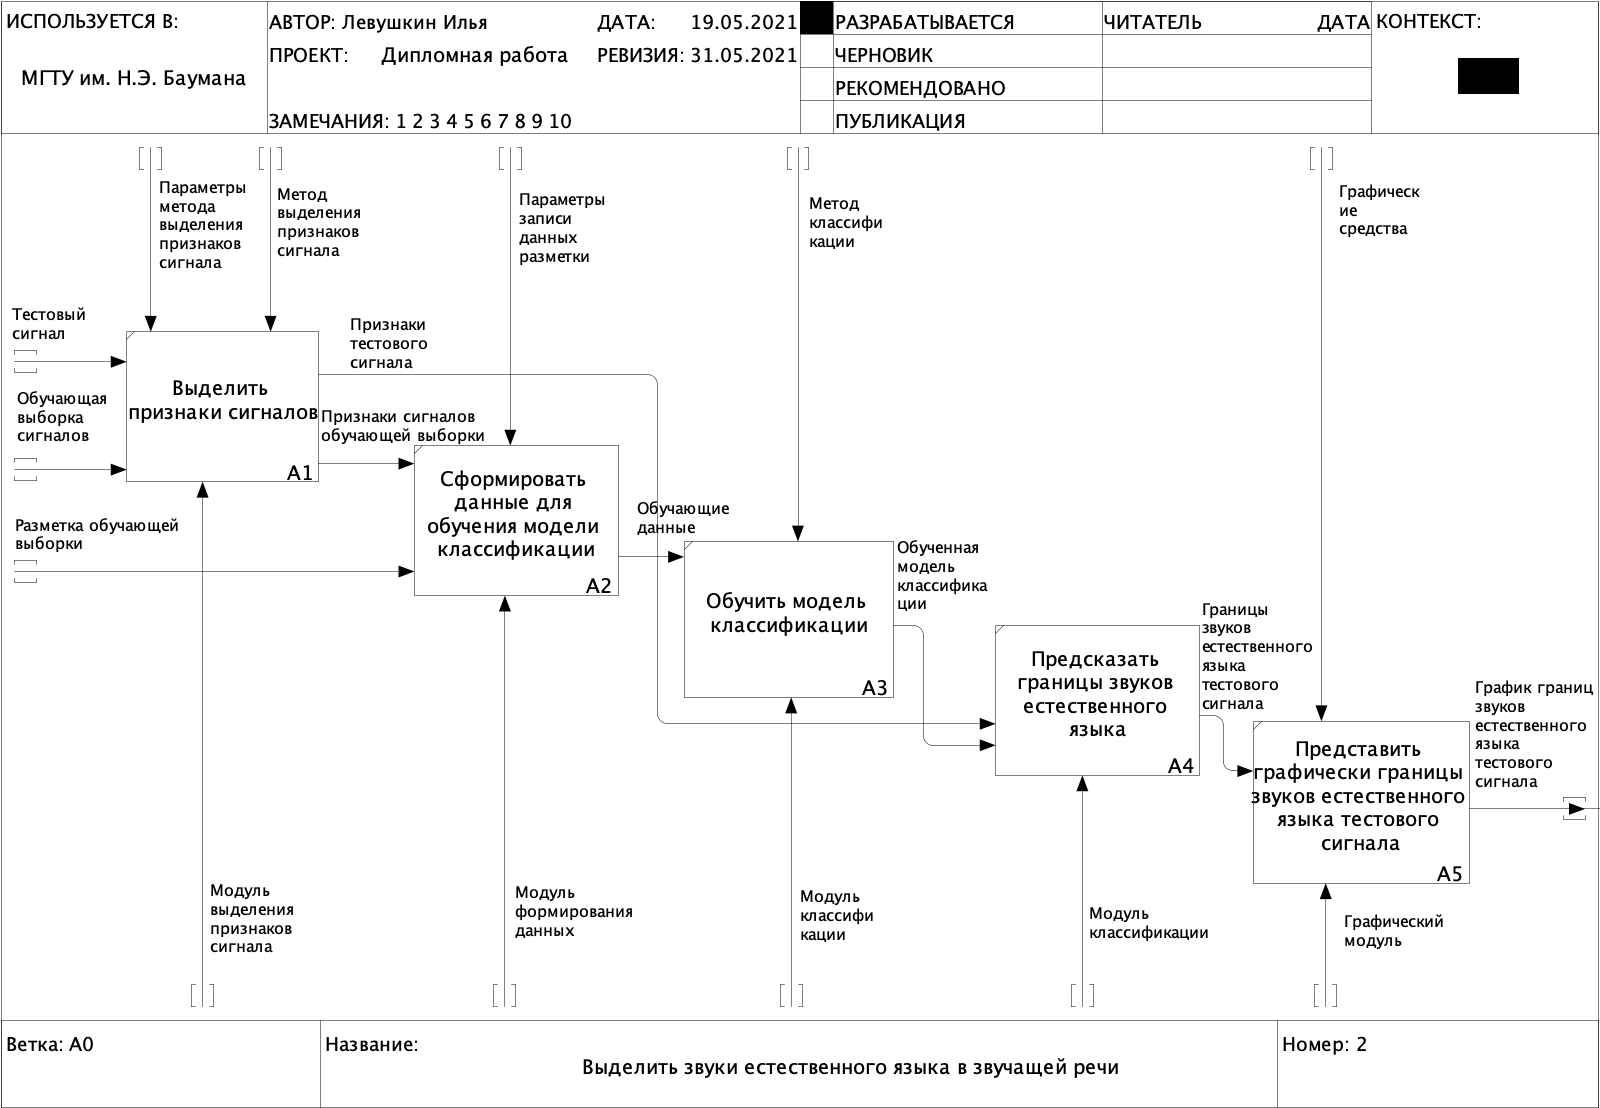
\includegraphics[scale = 0.3]{img/ramus_A1-A5.png}}
		\end{center}
		\caption{IDEF0 диаграмма разрабатываемого алгоритма.}
		\label{ris:ramus_A1-A5}
	\end{figure}

	\subsection{Выделение признаков речевого сигнала}\label{features_preprocessing}
	
	 В данной работе было решено использовать метод многомасштабного Вейвлет-анализа сигнала (раздел \ref{anal_summary}), в результате чего схема алгоритма выделения признаков речевого сигнала выглядит следующим образом \cite{vevlet_1}:

	\begin{enumerate}
		\item В качестве предобработки сигнал нормализуется: все отсчеты делятся на максимальное значение, для установки единых пороговых значений для любых входных сигналов;
		\item Входной сигнал разбивается на фреймы по $n_{frame}$ отсчётов при частоте дискретизации $sr$ с перекрытием $hop$.
		\item Каждый фрейм накрывается окном Хэмминга для устранения дефектов на краях;
		\item К каждому фрейму применяется вейвлет-преобразование в базисе $base$. Используется разложение до $k$-го уровня декомпозиции;
		\item Для каждого уровня декомпозиции определяется энергия, как сумма
		квадратов значений коэффициентов детализации E \cite{rem}.
	\end{enumerate}

	Ниже приведены варьируемые параметры, поступающие на вход модулю выделения принаков сигнала:
	
	\begin{itemize}
		\item $n_{frame}$ - количество отсчетов в одном фрейме (по умолчанию - 2500);
		\item $sr$ - частота дискретизации сигнала, Гц (по умолчанию - 16000);
		\item $hop$ - размер перекрытия фрейма другим фреймом, \% (по умолчанию - 40);
		\item $base$ - базисная функция вейвлет-пребразования (по умолчанию - Вейвлет Добеши 8);
		\item $k$ - уровень декомпозиции сигнала (по умолчанию - 6).
	\end{itemize}
	
	\subsection{Формирование данных для обучения модели классификации}
	
	Из формализованной постановки задачи классификации (раздел \ref{formal_classification}) следует, что для обучения модели классификации необходимо сформировать обучающую выборку таким образом, чтобы каждому вектору признаков \linebreak $(x^1, x^2, ..., x^d)$ объекта $x$ множества $X^m$ соответствовало единственное значение ответа $y = y(x)$ множества $Y^m$:
	
	\begin{equation}
		X^m = {(x_1, y_1), ..., (x_m, y_m)}.
	\end{equation}
	
	В терминах данной задачи это означает, что каждому вектору признаков речевого сигнала за определенный промежуток времени $t$ требуется сопоставить ответ на вопрос - \textit{является ли данный интервал $t$ границей межфонемного перехода?}
	
	Говоря формально, требуется сформировать список ответов $Y^m$, элементы $y_i$ которого принимают значения $\{0, 1\}$:
	
	\begin{itemize}
		\item 1 - в случае если объект $x_i$ (вектор признаков речевого сигнала на интервале времени $t_i$) является границей межфонемного перехода;
		\item 0 - в противном случае.
	\end{itemize}

	Исходя из приведенных выше рассуждений, схема формирования данных для модели классификации выглядит следующим образом:
	
	\begin{enumerate}
		\item Извлечение границ (моментов времени) $T = (t_1,...,t_s)$ межфонемных переходов из файла с обучающей выборкой в соответствии с ее параметрами записи данных;
		\item Избавление от зашумленных данных путем усреднения значений $t_i$ и $t_{i+1}$ при условии, что $t_{i+1} - t_i < lim_{phonem}$, где $lim_{phonem}$ - минимальный порог длительности фонемы (если расстояние между соседними значениями $t$ меньше порогового, то заменяем их средним значением);
		\item Преобразование границ межфонемных переходов $T = (t_1, ..., t_s)$ в список ответов $Y = (y_1,...,y_m)$, где $y_i \in {0, 1}$. 
	\end{enumerate}
	
	\subsection{Обучение модели классификации}\label{features_classification}
	
	В данной работе было решено использовать метод опорных векторов SVM (раздел \ref{anal_summary}) в качестве алгоритма классификации.
	
	Ниже приведены настраиваемые параметры метода:
	
	\begin{itemize}
		\item kernel - ядро SVM, задает функцию разделяющей гиперплоскости. Наиболее популярные ядра - linear (линейная функция), rbf (радиально-базисная функция), poly (полиномиальная функция). В данной реализации метода выбрано по умолчанию ядро rbf;
		\item C - параметр регуляризации. Варьирование этого параметра позволяет понизить уровень переобучения модели, поскольку он контролирует соотношение между гладкой границей и корректной классификацией рассматриваемых точек. По умолчанию - 1.0;
		\item gamma - <<ширина>> ядра. Варьирование этого параметра также позволяет понизить уровень переобучения модели для нелинейных ядер. По умолчанию равен $\frac{1}{n_{features} * X_{var}}$;
		\item class\_weight - параметр, позволяющий варьировать размер штрафа при \linebreak неудачном выборе класса. Используется при несбалансированной выборке классов. По умолчанию равен balanced, то есть устанавливает штраф за ошибку выбора класса пропорционально размеру этого класса в обучающей выборке. Применяется, поскольку в данной задаче классы имеют значительный дисбаланс (интервалов времени, на которых присутствуют границы межфонемных переходов, значительно меньше чем тех, на которых их нет).
	\end{itemize}

	
	\subsection{Структура ПО}
	
	Архитектура ПО использует внутри себя принципы архитектурного паттерна MVC (Model-View-Controller), который разделяет общую структуру кода на три отдельных компонента:
	\begin{itemize}
		\item модель - предоставление данных конкретным элементам системы;
		\item представление - реагирует на изменение данных в системе и обеспечивает их отображение пользователю;
		\item контроллер - точка входа для доступа к модели и представлению. Контроллер обрабатывает действия пользователя, после чего отдает сигнал модели о необходимости каким-либо образом измениться.
	\end{itemize}

	При использовании MVC достигается возможность разделения компонентов работы с данными, пользовательским интерфейсом и логикой взаимодействия пользователя с приложением, в результате чего модификация одного из компонентов оказывает минимальное воздействие на остальные.
	
	\begin{figure}[h!]
		\begin{center}
			{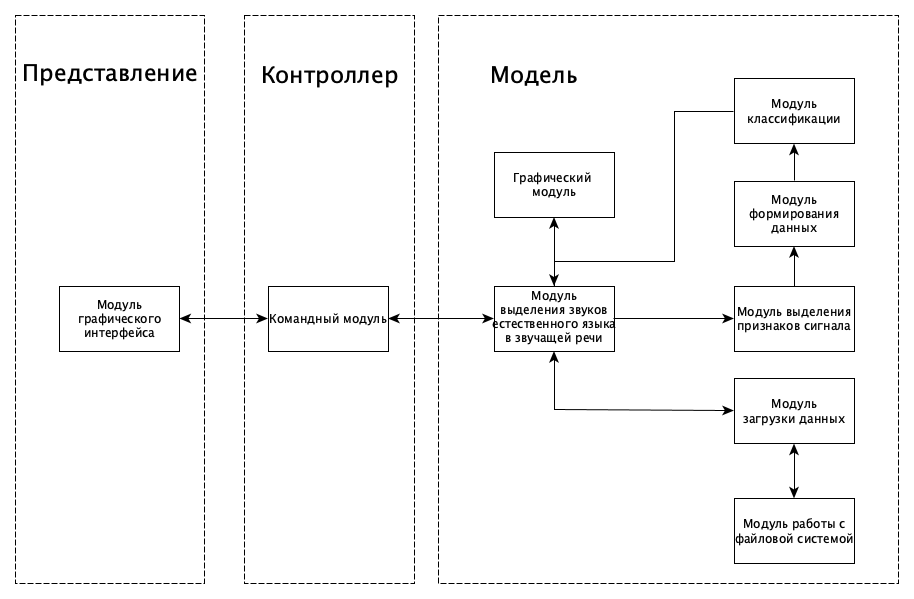
\includegraphics[scale = 0.5]{img/mvc.png}}
		\end{center}
		\caption{Архитектура программного обеспечения.}
		\label{ris:mvc}
	\end{figure}

	Графический интерфейс предоставляет пользователю возможность взаимодействия с разработанным ПО. 
	
	Доступный функционал:
	\begin{itemize}
		\item возможность выбрать аудио-файл (формат mp3) для тестирования метода, аудио-файлы (формат mp3) и разметку (формат csv) для обучения модели классификации;
		\item возможность обучить модель классификации;
		\item возможность сохранить обученную модель классификации в файл (формат pkl);
		\item возможность загрузить обученную модель классификации из файла (формат pkl);
		\item возможность определения границ межфонемных переходов выбранного сигнала для тестирования;
		\item сохранение результатов в файл (формат csv);
		\item графическое отображение результатов в диалоговом окне.
	\end{itemize}
	
	Модули, изображенные на рисунке \ref{ris:mvc}, содержат необходимые классы и методы, выполняющие основную логику приложения.
	
	Ниже приведено описание основных классов, представленных на рисунке \ref{ris:uml}.
	
	\begin{itemize}
		\item Классы \textit{MainView, ResultView, TeachModelView} - обрабатывают логику запросов пользователя к графическому интерфейсу приложения;
		\item Класс \textit{MainController} агрегирует в себе классы \textit{MainView, ResultController, TeachModelController, SoundsExtractionModule}. Является точкой входа в приложение и отвечает за распределение задач от \textit{MainView} к 
		
		\textit{SoundsExtractionModule} и по своим контроллерам - \textit{ResultController},
		
		\textit{TeachModelController};
		\item \textit{ResultController и TeachModelController} отвечают за распределение задач от \textit{ResultView и TeachModelView к SoundsExtractionModule};
		\item \textit{SoundsExtractionModule} агрегирует в себе все модули: \textit{GraphModule},
			
		\textit{FeatureExtractionModule, DataPreprocessingModule, ClassificationModule и LoadDataModule}. Отвечает за распределение задач от контроллеров по модулям;
		\item \textit{LoadDataModule} отвечает за работу с файловой системой. Осуществляет загрузку и выгрузку данных: \textit{test\_signal, train\_signals, train\_markups, model};
		\item \textit{ClassificationModule} отвечает за обучение модели и осуществление ею предсказаний;
		\item \textit{DataPreprocessingModule} отвечает за предобратку данных. Формирует обучающую и тестовую выборки для \textit{ClassificationModule};
		\item \textit{FeatureExtractionModule} отвечает за извлечение признаков из сигналов.
	\end{itemize}
	
	\begin{figure}[h!]
		\begin{center}
			{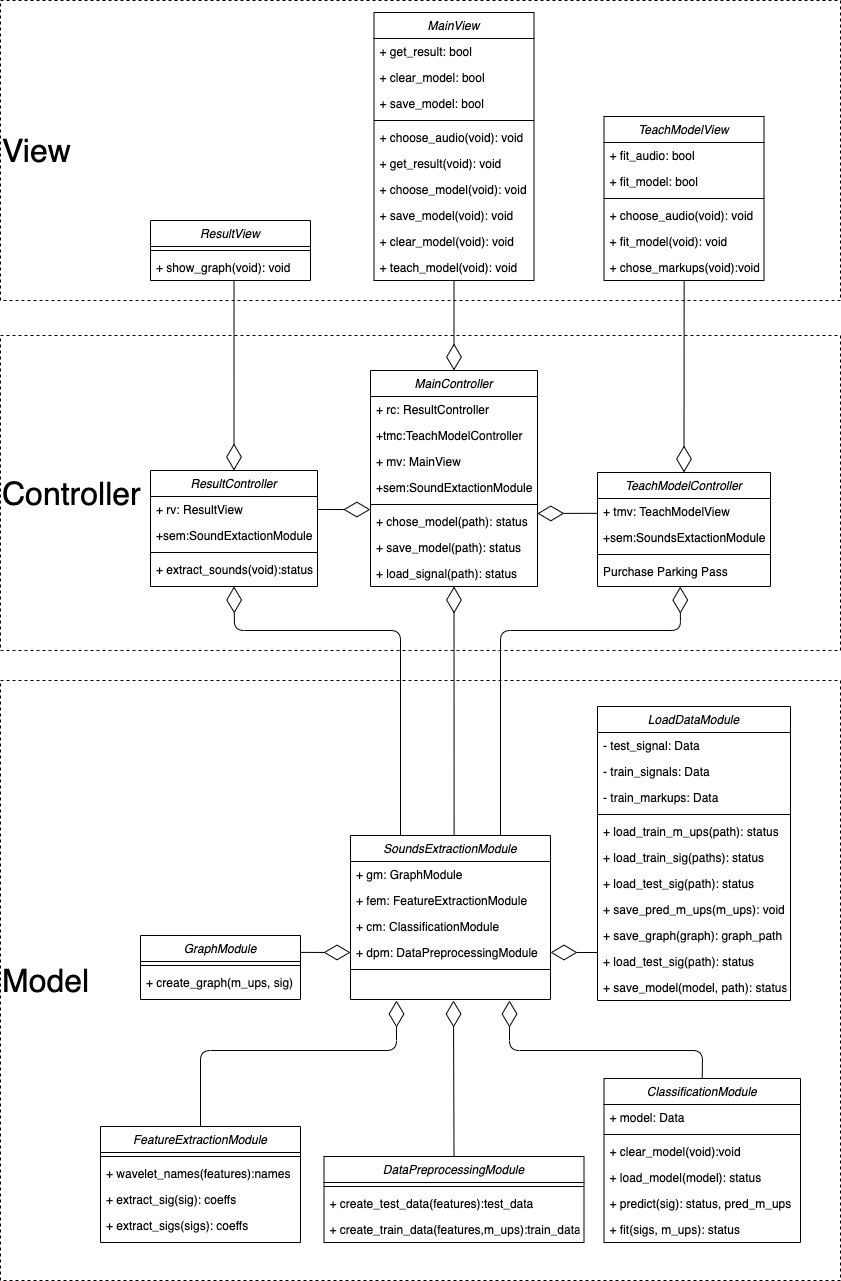
\includegraphics[scale = 0.4]{img/uml.png}}
		\end{center}
		\caption{Схематичное представление архитектуры программного обеспечения.}
		\label{ris:uml}
	\end{figure}

	\subsection{Описание формата входных и выходных данных}
	
	Для обучения модели пользователь выбирает файлы аудио-сигналов (формат mp3) и разметку этих аудио-файлов (формат csv). Разметка аудио-файлов представляет из себя таблицу со столбцами \textit{filename, start, end, intervals}, где
	
	\begin{itemize}
		\item filename - имя аудио-файла;
		\item start - начало фонемы;
		\item end - конец фонемы;
		\item intervals - список границ, на которых был размечен аудио-файл.
	\end{itemize}

	Вместо обучения пользователь может загрузить файл обученной модели (формат pkl).
	
	Для тестирования модели пользователь выбирает файл с аудио-сигналом (формат mp3).
	
	{\bf На выходе} пользователь получает график границ межфонемных переходов, выведенный на экран и сохраненный в файл (формат png), список выделенных границ межфонемных переходов, сохраненных в файл (формат csv).
	
	Также, пользователь имеет возможность сохранить обученную модель в файл (в формате pkl).
	
	\subsection{Выводы}
	
	В результате написания конструкторского раздела были решены следующие задачи:
	\begin{itemize}
		\item спроектирован метод выделения звуков естественного языка в звучащей речи;
		\item разработан алгоритм, реализующий данный метод, и приведено подробное его описание;
		\item спроектирована архитектура системы для проверки работоспособности метода;
		\item описаны формат входных и выходных данных и структура разрабатываемого программного обеспечения.
	\end{itemize}
		
	\pagebreak
	
	\section{Технологическая часть}
	
	\subsection{Выбор языка программирования}
	
	В качестве языка программирования был выбран язык программирования \textit{Python3} - объектно-ориентированный интерпретируемый язык программирования высокого уровня \cite{python}.
	
	Преимуществами данного языка являются:
	
	\begin{itemize}
		\item встроенные типы данных высокого уровня: списки, словари, строки и другие;
		\item объектно-ориентированность - язык предоставляет удобный интерфейс создания и использования объектов;
		\item широко используется в научных исследованиях, так как обладает большим объемом различных библиотек для решения прикладных задач из различных областей, включая такие области как цифровая обработка сигналов, машинное обучение, работа со сложными математическими вычислениями и большим объемом данных.
	\end{itemize}
	
	\subsection{Выбор используемых библиотек}
	
	Спроектированный метод выделения звуков естественного языка звучащей речи состоит из двух этапов (раздел \ref{segment}):
	\begin{enumerate}
		\item выделение признаков сигнала;
		\item определение межфонемных переходов на основе выделенных признаков сигнала.
	\end{enumerate}
	
	{\bf Первый этап} подразумевает работу с аудио-сигналами, а именно - загрузка аудио-файлов, дискретизация сигнала, разделение сигнала на перекрывающиеся участки - фреймы.
	
	Для решения этих задач было решено использовать библиотеку \textit{Librosa} \cite{librosa} - модуль python, предоставляющий удобный интерфейс для анализа звуковых сигналов.
	
	В качестве модуля выделения признаков сигнала был выбран \textit{Многомасштабный Вейвлет-анализ} (раздел \ref{anal_summary}). Для решения этой задачи была выбрана библиотека \textit{pywt} \cite{pywt} - модуль python, предоставляющий необходимый инструментарий для применения вейвлет-преобразования на дискретном сигнале.
	
	На {\bf втором этапе} для определения границ между основными лингвистическими элементами языка было решено применить метод классификации машинного обучения (раздел \ref{formal_classification}) - метод опорных векторов SVM \cite{svm}. Наиболее популярным подходом к решению задач классификации является использование библиотеки \textit{Scikit-Learn} \cite{scikit-learn} в связке с такими инструментами как \textit{Pandas} \cite{pandas}, \textit{NumPy} \cite{numpy} и \textit{Matplotlib} \cite{matplotlib}. Такой подход позволяет наиболее эффективно использовать объем доступной памяти и процессорное время, предоставляемое системой.
	
	\begin{itemize}
		\item \textit{Pandas} - библиотека python для обработки и анализа больших данных. Использует объекты \textit{NumPy} и предоставляет специальные структуры данных и операции для манипулирования числовыми таблицами и временными рядами;
		\item \textit{NumPy} - библиотека python, добавляющая поддержку больших многомерных массивов и матриц, вместе с большой библиотекой высокоуровневых и быстрых математических функций для операций с этими массивами;
		\item \textit{Matplotlib} - библиотека python, использующаяся для построения графиков и диаграмм. Использует объекты \textit{NumPy} и предоставляет объектно- \linebreak ориентированный интерфейс для данных, отображая получившиеся результаты с помощью встроенных графических библиотек.
	\end{itemize}

	Графический интерфейс, используемый пользователем был написан при помощи библиотеки \textit{PyQt5} \cite{pyqt5} - графической библиотеки python, предоставляющей возможность создавать графические интерфейсы для пользователя. Данная библиотека использует понятную структуру наследования и предлагает \linebreak объектно-ориентированные решения с логической иерархией между объектами.
	
	\subsection{Выбор среды разработки}
	
	В качестве среды разработки было решено использовать \textit{PyCharm} \cite{pycharm}, имеющий доступный интерфейс, а также большое количество полезных функций и плагинов, упрощающих процесс разработки.
	
	Поскольку \textit{PyCharm} нативно поддерживает Python, данная среда разработки выполняет большое количество рутинных действий за разработчика. Среда снабжена отладчиком, необходимым для разработки ПО. Также, среда предоставляет возможность удобного рефакторинга кода, меняя все зависимости во всем проекте.
	
	\subsection{Пользовательский интерфейс}
	
	Пользователь взаимодействует с графическим интерфейсом ПО курсором мыши и клавиатурой.
	
	Ниже приведено описание взаимодействия пользователя с графическим интерфейсом ПО.
	\begin{itemize}
		\item {\bf Обучение модели.}
		
		Для обучения модели классификации, пользователю необходимо нажать на кнопку \textit{Обучить модель классификации}. 
		
		\begin{figure}[h!]
			\begin{center}
				{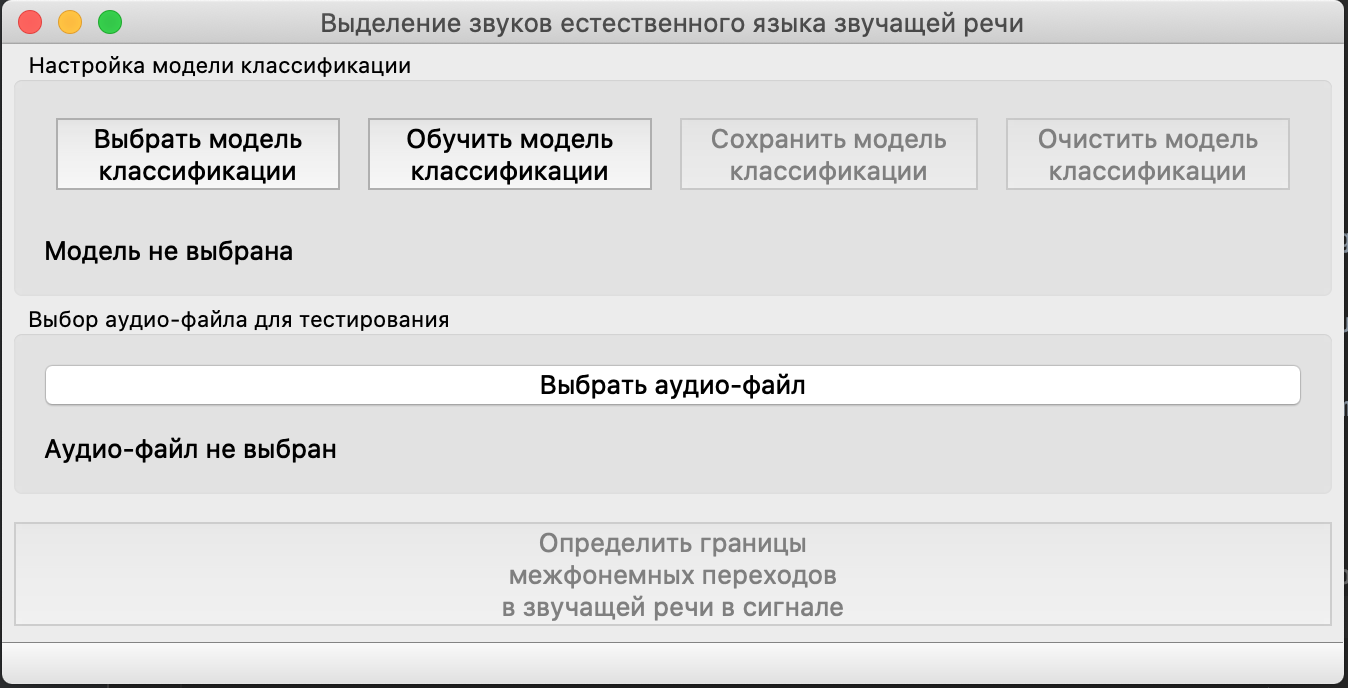
\includegraphics[scale = 0.65]{img/start.png}}
			\end{center}
			\caption{Главное меню.}
			\label{ris:start}
		\end{figure}
		
		В открывшемся диалоговом окне необходимо выбрать файл-разметки аудио-сигналов для обучения модели, нажав на кнопку \textit{Выбрать разметку для обучения}. Затем выбрать аудио-файлы для обучения модели, нажав на кнопку \textit{Выбрать аудио-файлы для обучения}. После загрузки файлов, нажать \linebreak кнопку \textit{Обучить модель}, дождаться конца обучения и нажать кнопку \textit{ОК}.
		
		\newpage
		
		\begin{figure}[h!]
			\begin{center}
				{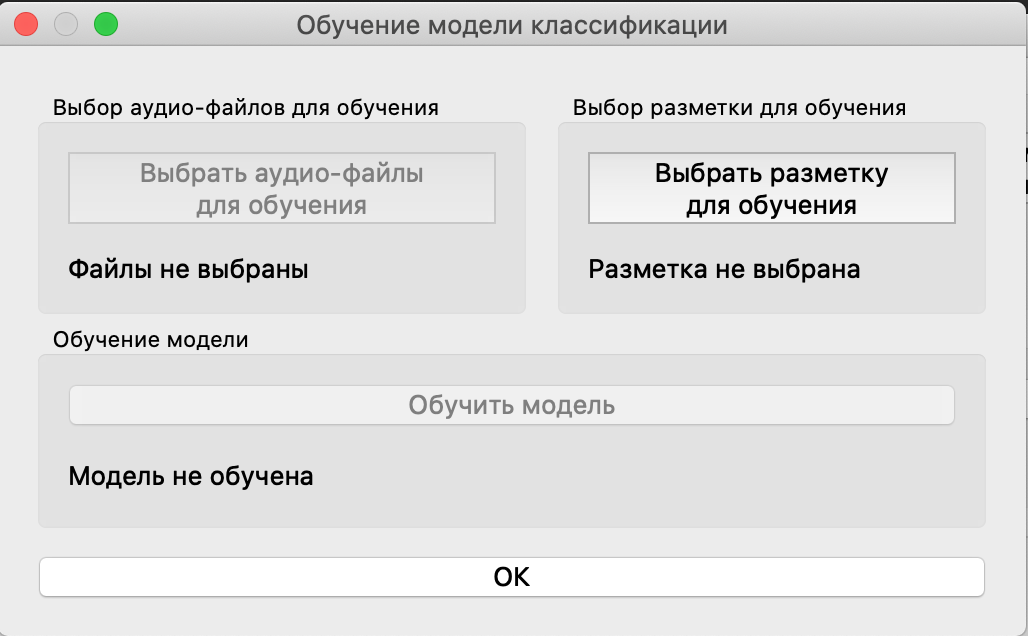
\includegraphics[scale = 0.8]{img/teach.png}}
			\end{center}
			\caption{Обучение модели.}
			\label{ris:teach}
		\end{figure}
		
		\item {\bf Сохранение модели.}
		
		После обучения модели появляется возможность сохранить модель. Для этого необходимо нажать на кнопку \textit{Сохранить модель классификации}.
		
		\begin{figure}[h!]
			\begin{center}
				{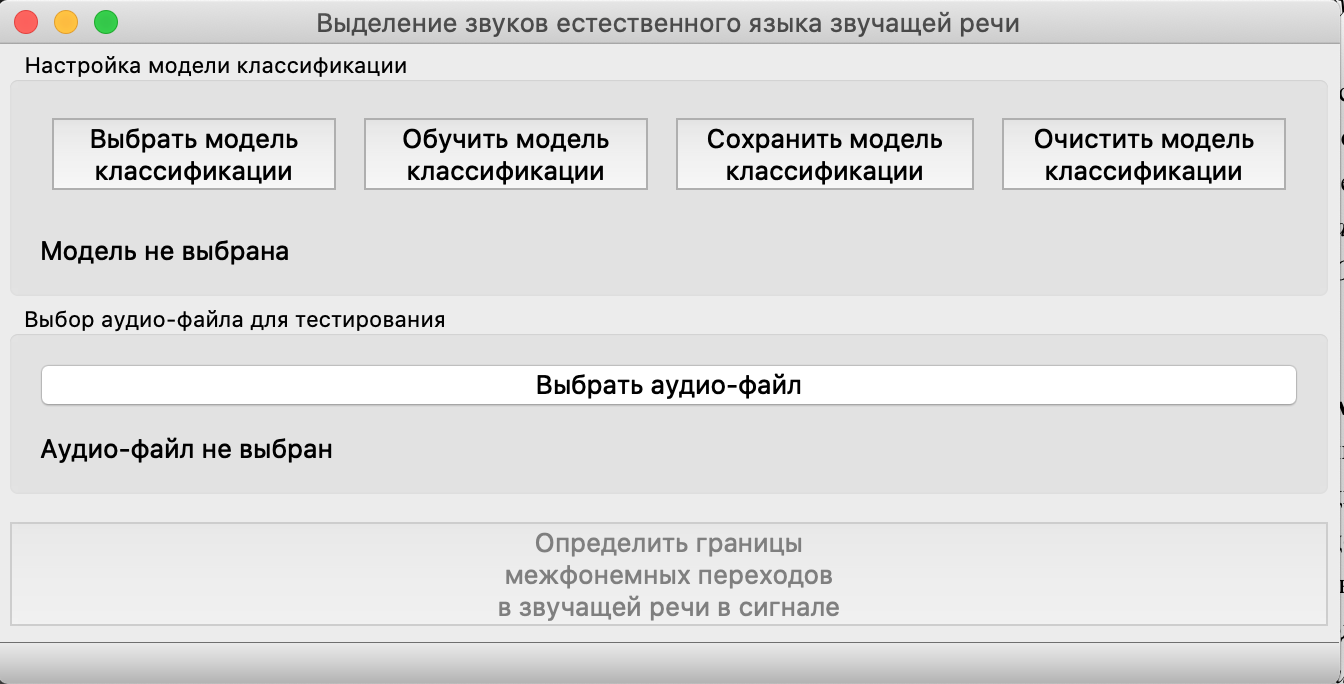
\includegraphics[scale = 0.6]{img/save_model.png}}
			\end{center}
			\caption{Сохранение модели.}
			\label{ris:save_mode}
		\end{figure}
		
		\item {\bf Загрузка модели.}
		
		Вместо обучения модели пользователь имеет возможность загрузить файл обученной модели. Для этого необходимо нажать на кнопку \textit{Выбрать модель классификации}.
		
		\item {\bf Сброс модели.}
		
		После загрузки или обучения модели классификации у пользователя появляется возможность сбросить модель. Для этого необходимо нажать на кнопку \textit{Очистить модель классификации}.
		
		\item {\bf Выбор аудио-файла.}
		
		Пользователь имеет возможность загрузить аудио-файл для тестирования ПО. Для этого необходимо нажать на кнопку \textit{Выбрать аудио-файл}.
		
		\item {\bf Выделение звуков естественного языка звучащей речи}
		
		Для получения результатов предсказания модели пользователь должен нажать на кнопку {\bf Определить границы межфонемных переходов звучащей речи в сигнале} после выбора тестового аудио-файла и обучения/загрузки модели.
		
		\begin{figure}[h!]
			\begin{center}
				{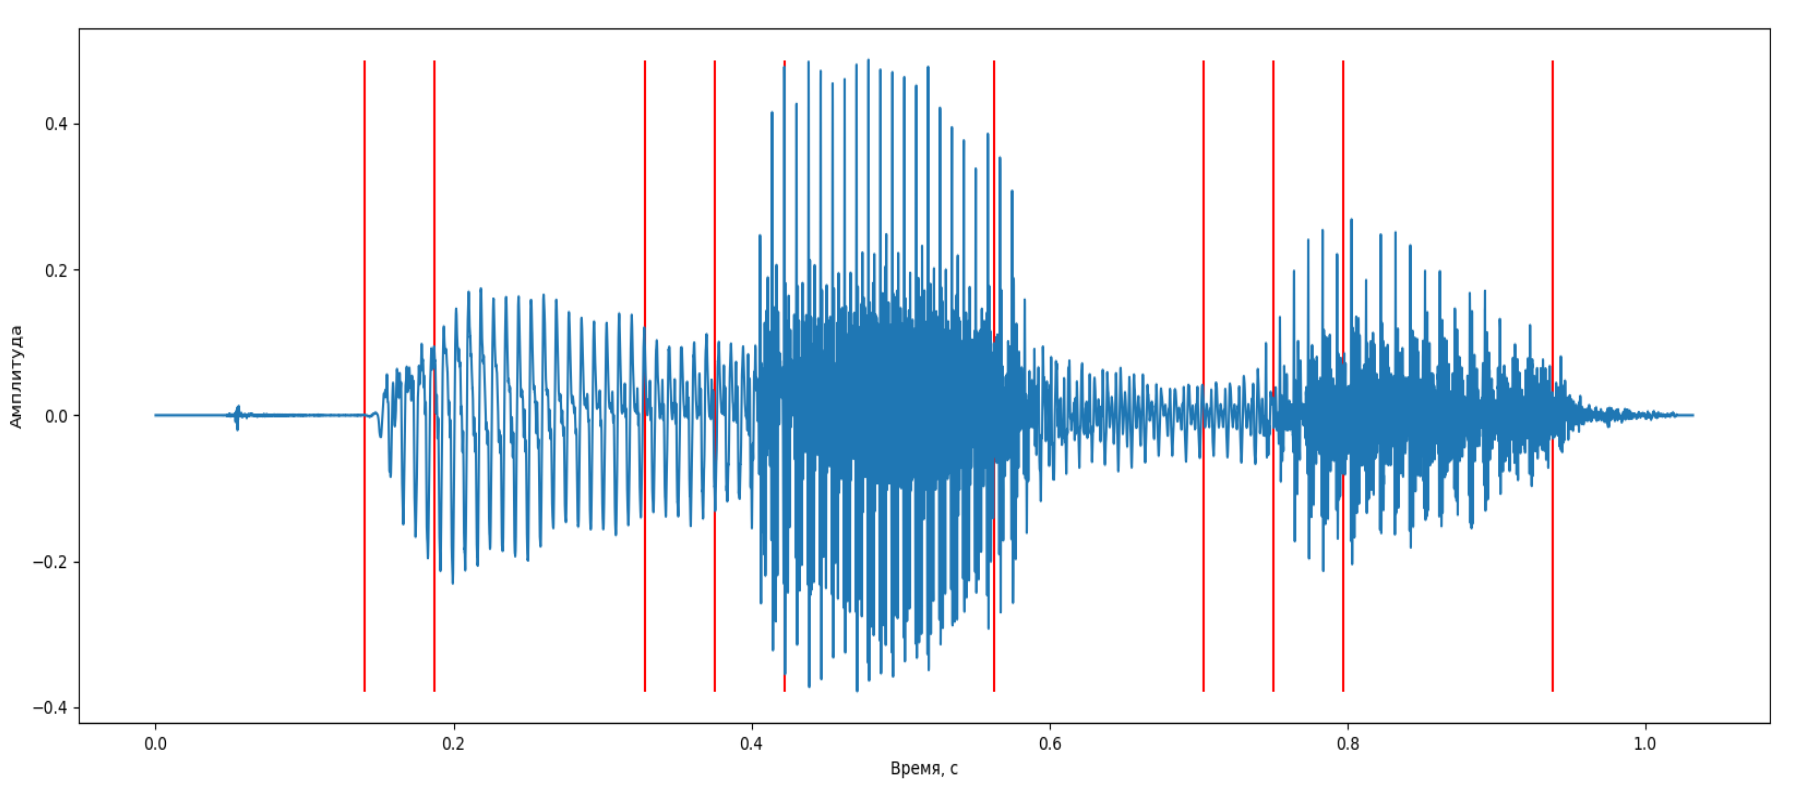
\includegraphics[scale = 0.5]{img/get_results.png}}
			\end{center}
			\caption{Выделение границ межфонемных переходов звучащей речи в сигнале.}
			\label{ris:get_results}
		\end{figure}
	\end{itemize}
	
	\subsection{Реализация}
	
	Ниже приведены листинги кода реализаций некоторых компонентов ПО: блоков работы с данными - Model, блока работы с пользовательским интерфейсом - View, блока логики взаимодействия пользователя с приложением - Controller (полный листинг кода разработанного ПО в разделе \textit{ПРИЛОЖЕНИЕ А}).
	
	{\bf MainView} - логика запросов пользователя к графическому интерфейсу главного экрана приложения.
		
		\begin{lstlisting}[caption=MainView]
from PyQt5 import uic
from PyQt5.QtCore import pyqtSlot, Qt
from PyQt5.QtWidgets import QMessageBox, QMainWindow, QFileDialog


class MainWindow(QMainWindow):
	def __init__(self, in_controller):
		super(MainWindow, self).__init__()
		self.ui = uic.loadUi("view/main_view/main_window.ui", self)
		self.controller = in_controller
		self.ui.get_result_button.setEnabled(False)
		self.ui.clear_model_button.setEnabled(False)
		self.ui.save_model_button.setEnabled(False)
	
	@pyqtSlot(name='on_choose_model_button_clicked')
	def choose_model(self):
		filename, _ = QFileDialog.getOpenFileName(self, 'Выберите модель для загрузки',
		'./Data/models/', 'Model File(*.pkl)')
		if len(filename) > 0:
		status = self.controller.choose_model(filename)
		if status == 'Модель успешно загружена':
			self.ui.clear_model_button.setEnabled(True)
			self.try_enable_get_result_btn()
		else:
			msgBox = QMessageBox()
			msgBox.setStandardButtons(QMessageBox.Ok)
			msgBox.setIcon(QMessageBox.Critical)
			msgBox.setText(status)
			msgBox.exec()
	
	@pyqtSlot(name='on_teach_model_button_clicked')
	def teach_model(self):
		self.controller.launch_teach_model_view()
		self.ui.clear_model_button.setEnabled(True)
		self.ui.save_model_button.setEnabled(True)
	\end{lstlisting}
	
	\newpage

	\begin{lstlisting}[caption=MainView Продолжение]
	@pyqtSlot(name='on_save_model_button_clicked')
	def save_model(self):
		filename, _ = QFileDialog.getSaveFileName(self, 'Сохранить модель',
		'./Data/models/', 'Model File (*.pkl)')
		if len(filename) > 0:
			status = self.controller.save_model(filename)
			msgBox = QMessageBox()
			msgBox.setStandardButtons(QMessageBox.Ok)
			if status == 'Модель успешно сохранена':
				msgBox.setIcon(QMessageBox.Information)
				msgBox.setText(status)
				self.ui.save_model_button.setEnabled(False)
			else:
				msgBox.setIcon(QMessageBox.Critical)
				msgBox.setText(status)
			msgBox.exec()
	
	@pyqtSlot(name='on_clear_model_button_clicked')
	def clear_model(self):
		self.controller.clear_model()
		self.ui.clear_model_button.setEnabled(False)
		self.ui.get_result_button.setEnabled(False)
	
	
	@pyqtSlot(name='on_choose_test_audio_button_clicked')
	def choose_test_audio(self):
		filename, _ = QFileDialog.getOpenFileName(self, 'Выберите mp3-файл для тестирования',
		'./Data/test/', 'Audio File(*.mp3)')
		if len(filename) > 0:
			status = self.controller.load_test_signal(filename)
			self.ui.choose_test_audio_label.setText(status)
			self.try_enable_get_result_btn()
	
	@pyqtSlot(name='on_get_result_button_clicked')
		def get_result(self):
		self.controller.launch_result_view()
		\end{lstlisting}
		
		{\bf MainController} - точка входа в приложение. Отвечает за распределение задач от \textit{MainView} к \textit{SoundsExtractionModel} и по агрегируемым в себе контроллерам - \textit{ResultContoller}, \textit{TeachModelController}.
		
		\newpage
		
		\begin{lstlisting}[caption=MainController]
class MainController:
	def __init__(self):
		self.main_window = MainWindow(self)
		self.main_window.show()
		self.sounds_extraction_module = SoundsExtractionModule()
		
		# инициализация teach_model_controller
		self.teach_model_controller = TeachModelController(self, self.sounds_extraction_module)
	
	# инициализация result_controller
		self.result_controller = ResultController(self, self.sounds_extraction_module)
	
	def launch_teach_model_view(self):
		self.teach_model_controller.show_window()
	
	def teach_model_window_closed(self):
		self.main_window.try_enable_get_result_btn()
	
	def launch_result_view(self):
		self.result_controller.show_window()
	
	def clear_model(self):
		self.sounds_extraction_module.clear_classification_model()
	
	def load_test_signal(self, filename):
		return self.sounds_extraction_module.load_test_signal(filename)
	
	def choose_model(self, path):
		return self.sounds_extraction_module.choose_model(path)
	
	def save_model(self, path):
		return self.sounds_extraction_module.save_classification_model(path)
		\end{lstlisting}
		
		{\bf FeatureExtractionModule} - модуль, отвечающий за извлечение признаков из сигналов.
		
		\newpage
		\begin{lstlisting}[caption=FeatureExtractionModule]
from scipy import signal
from pywt import wavedec

from model.params.audio_params import AudioParams

class FeatureExtractionModule:
	
	@staticmethod
	def get_t_between_frames(frames_coeffs, offset):
		t_values = []
		cur_time = offset
		dt = AudioParams.frame_sz() * AudioParams.hop_part() / AudioParams.sr()
		for i in range(len(frames_coeffs)):
			t_values.append(cur_time)
			cur_time += dt
		return np.array(t_values)
	
	# получает массив сигналов: [[path, signal],...], возвращает словарь признаков: {path: feature}
	def extract_from_signals(self, sigs):
		res = []
		for path_sig in sigs:
			res.append([path_sig[0], self.extract_from_signal(path_sig[1])])
		return res
	
	# получает на вход signal, возвращает признаки signal
	def extract_from_signal(self, sig):
		# разбитие сигнала на фреймы
		frames_sig = self._splitting_signal_on_frames(sig, AudioParams.frame_sz(), AudioParams.hop_part())
		
		# устранение деффекта на краях с помощью оконной функции Хамминга
		frames_hamming_sig = self._hamming_func(frames_sig, AudioParams.frame_sz())
		
		# применение вейвлет-преобразования
		frames_coeffs = self._frames_wavelet(frames_hamming_sig, AudioParams.wavelet(), AudioParams.wavelet_level())
		
		return frames_coeffs
	\end{lstlisting}
	\newpage
	\begin{lstlisting}[caption=FeatureExtractionModule Продолжение]
	def _splitting_signal_on_frames(self, descrete_sig, frame_sz, hop_part):
		frames = librosa.util.frame(descrete_sig, frame_length=frame_sz, hop_length=int(hop_part * frame_sz), axis=0)
		return frames
	
	def _hamming_func(self, frames_signal, frame_sz):
		w = signal.windows.hamming(frame_sz, sym=True)
		return np.array([w * frame for frame in frames_signal])
	
	def _wavelet_conv(self, sig, method, level):
		return np.array(wavedec(sig, method, level=level))
	
	def _frames_wavelet(self, frames_signal, method, level):
		return np.array([self._wavelet_conv(sig, method, level) for sig in frames_signal], dtype=object)

		\end{lstlisting}
	{\bf DataPreprocessingModule} - модуль, формирующий обучающую и тестовую выборки для \textit{ClassificationModule}.
	\begin{lstlisting}[caption=DataPreprocessingModule]
import numpy as np
from itertools import chain
import pandas as pd
import ast

from model.feature_extraction_module.feature_extraction_module import FeatureExtractionModule
from model.params.markups_params import MarkupsParams
from model.params.audio_params import AudioParams

class DataPreprocessingModule:

	# получает на вход signal, возвращает признаки signal
	def create_test_data(self, features):
		features_names = FeatureExtractionModule.get_wavelet_columns_names(features[0])
		res_data = []
		for feature in features:
			res_data.append(list(chain(*feature)))
		return pd.DataFrame(res_data, columns=features_names)
	\end{lstlisting}
	\begin{lstlisting}[caption=DataPreprocessingModule Продолжение]
	# получает массив признаков [[path, feature],...], разметку в pandas с колонками: ['recordname', 'start', 'end']
	# возвращает обучающую выборку в pandas формате: [feature, feature, ..., y], y = {0,1}
	def create_train_data(self, features, df_markups):
		# получаем названия признаков
		features_names = FeatureExtractionModule.get_wavelet_columns_names(features[0][1][0])
		features_names.append('y')
		res_data = []
		for path, frames_coeffs in features:
			filename = self._get_filename_from_path(path)
			for interval in ast.literal_eval(df_markups[df_markups[MarkupsParams.filename()] == filename]
			.intervals.iloc[0]):
				# получаем временные промежутки между фреймами
				t_positions_between_frames = FeatureExtractionModule.get_t_between_frames(frames_coeffs, interval[0])
				# формируем список Вейвлет-коэффициентов (n) - один фрейм
				# (длина списка - t_positions_between_frames) и добавляем к нему y={0,1}
				y = np.zeros(frames_coeffs.shape[0])
				borders = self._borders_preprocessing(
				df_markups[df_markups[MarkupsParams.filename()] == filename],
				MarkupsParams.start_end()[0], MarkupsParams.start_end()[1])
				# оставляем только те границы, что лежат в интервале interval
				borders = self._filter_borders(borders, interval)
				for border in borders:
					for t_pos in range(len(t_positions_between_frames)):
					if t_positions_between_frames[t_pos] > border:
						y[t_pos] = 1.
						break
				# преобразуем frames_coeffs
				res_data_i = []
				for frame, y_i in zip(frames_coeffs, y):
					lst_i = list(chain(*frame))
					lst_i.append(y_i)
					res_data_i.append(lst_i)
				res_data.extend(res_data_i)
		return pd.DataFrame(res_data, columns=features_names)
	\end{lstlisting}
	{\bf ClassificationModule} - модуль, отвечающий за обучение модели и осуществление ею предсказаний.
	\begin{lstlisting}[caption=ClassificationModule]
from model.data import Data
from model.params.classification_params import ClassificationParams

class ClassificationModule:
	def __init__(self, in_data_preprocessing_module, in_feature_extraction_module):
		self.data_preprocessing_module = in_data_preprocessing_module
		self.feature_extraction_module = in_feature_extraction_module
		self.params = ClassificationParams()
		self.model = Data('Модель не выбрана')
	
	def clear_model(self):
		self.model = Data('Модель не выбрана')
	
	def fit(self, signals, markups):
		if self.model.status == 'Модель обучена':
			return self.model.status
		try:
			# получает массив сигналов: [[path, audio],...], возвращает массив признаков: [[path, feature],...]
			features = self.feature_extraction_module.extract_from_signals(signals)
			# получает массив признаков [[path, feature],...],
			# разметку в pandas с колонками: ['filename', 'start', 'end']
			# возвращает обучающую выборку в pandas формате: [feature, feature, ..., y], y = {0,1}
			train_data = self.data_preprocessing_module.create_train_data(features, markups)
			
			self.params.model.fit(train_data.drop(axis=0, columns=['y']), train_data['y'].astype('int64'))
			
			self.model.data = self.params.model
			self.model.status = 'Модель обучена'
		except:
			return 'Ошибка обучения модели'
			return self.model.status
	\end{lstlisting}

	\newpage

	\begin{lstlisting}[caption=ClassificationModule Продолжение]
	# возвращает статус и список predicted_markups временных промежутков
	def predict(self, signal):
		if self.model.status != 'Модель обучена':
			return self.model.status
		try:
			features = self.feature_extraction_module.extract_from_signal(signal)
			# получает на вход признаки signal, возвращает pandas признаки с их именами
			test_data = self.data_preprocessing_module.create_test_data(features)
			predictions = self.model.data.predict(test_data)
			return 'Звуки успешно выделены', 	self._convert_predictions_to_time_list(predictions)
		except:
			return 'Ошибка! Не удалось выделить звуки', None
	\end{lstlisting}
	
	\subsection{Выводы}
	
	В данном разделе были выполнены следующие задачи:
	\begin{itemize}
		\item была реализована и протестировано программное обеспечение, спроектированное в разделе \ref{constructor}, для проверки работоспособности разработанного метода выделения звуков естественного языка в звучащей речи;
		\item было дано обоснование выбора языка программирования, среды разработки и используемых библиотек;
		\item было дано описание пользовательского интерфейса;
		\item были приведены листинги кода реализаций основных компонентов программного обеспечения.
	\end{itemize}
	\pagebreak
	
	\section{Исследовательская часть}
	
	\subsection{Формирование обучающей и тестовой выборок данных}
	
	В качестве данных для обучения и тестирования разработанного метода был задействован, размеченный студентами с кафедры Л4 и университета МГЛУ, речевой корпус. Данные представляли из себя аудио-файлы в mp3 формате и разметку к ним в формате json.
	
	В результате выполнения предобработки данных было получено 5806 объектов по 7 признаков в каждом. Предобработка данных выполнялась при следующих начальных параметрах (раздел \ref{features_preprocessing}):
	\begin{itemize}
		\item $n_{frame}$ = 2500;
		\item $sr$ = 16000 Гц;
		\item $hop$ = 40\%;
		\item $base$ = \textit{db4} (Вейвлет Добеши 8);
		\item $k$ = 6.
	\end{itemize}

	Ниже приведен вывод первых пяти сформированных объектов выборки.
	
	\begin{figure}[h!]
		\begin{center}
			{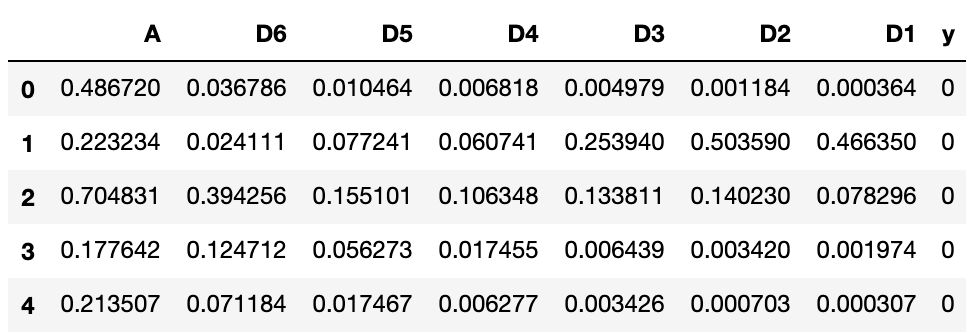
\includegraphics[scale = 0.6]{img/head.png}}
		\end{center}
		\caption{Формат сформированной выборки.}
		\label{ris:head}
	\end{figure}

	Под тестовую выборку было решено выделить всего 20\% объектов данных. Такой малый объем тестовых данных объясняется тем, что на этапе поиска оптимальных гиперпараметров модели планируется использовать кросс-валидацию \cite{cross-val} из 5 блоков, чтобы нейтрализовать эффект неравномерного распределения классов в тестовой выборке.
	
	\subsection{Метрики оценки качества моделей классификации}
	
	В сформированном датасете наблюдался дизбаланс классов - отношение количества объектов класса 1 (данный участок содержит в себе границу межфонемного перехода) к классу 0 равнялось$1:3$. В виду чего применение такой метрики оценки качества модели как \textit{доля правильных ответов алгоритма} - accuracy, будет давать неинформативные результаты.
	
	В виду чего было решено использователь другие метрики, независящие в той или иной степени от баланса классов в выборке.
	
	\subsubsection{precision и recall}
	
	Базовыми метриками для оценки качества модели классификации с несбалансированными классами являются \textit{precision} и \textit{recall}:
	
	\begin{equation}
		precision = \frac{TP}{TP+FP}
	\end{equation}

	\begin{equation}
		recall = \frac{TP}{TP+FN}
	\end{equation}

	Значения $TP, FP, FN$ получаются из таблицы сопряженности (таблица \ref{table:sopr}), строящейся на основе результатов классификации моделью и фактической принадлежности объектов к классам.
	
	\begin{center}
		\begin{longtable}[h!]{|p{0.3\linewidth}|p{0.3\linewidth}|p{0.3\linewidth}|}
			\hline
			{} & {$y = 1$} & {$y = 0$}\\
			\hline
			{$\hat{y} = 1$} & {True Positive (TP)} & {False Positive (FP)}\\
			\hline
			{$\hat{y} = 0$} & {False Negative (FN)} & {True Negative (TN)}\\
			\hline
			\caption{Таблица сопряженности.}
		\end{longtable}\label{table:sopr}
	\end{center}

	\begin{itemize}
		\item TP (True Positive) - верно классифицированные положительные объекты;
		\item TN (True Negative) - верно классифицированные отрицательные объекты;
		\item FN (False Negative) - неверно классифицированные отрицательные объекты;
		\item FP (False Positive) - неверно классифицированные положительные объекты.
	\end{itemize}

	В данной работе за положительный объект принимается класс 1 (объект содержит в себе границу межфонемного перехода), а за отрицательный - класс 0.
	
	Метрику \textit{precision} можно интерпретировать как долю объектов, названных классификатором положительными и при этом действительно являющимися положительными, а \textit{recall} показывает, какую долю объектов положительного класса из всех объектов положительного класса нашел алгоритм.
	
	\subsubsection{Коэффициент корреляции Мэтьюса} \label{met}
	
	При оптимизации гиперпараметров метода как правило используют одну метрику, улучшение результатов которой планируется увидеть на тестовой выборке.
	
	Одной из наиболее популярных метрик является F-мера - среднее гармоническое \textit{precision} и \textit{recall}:
	
	\begin{equation}
		F_1 = \frac{precision * recall}{precision + recall}
	\end{equation}

	Однако, данная метрика все еще может дать смещенную оценку предсказания, поскольку она не учитывает показатель $TN$.
	
	Наиболее оптимальным вариантом является использование \textit{Коэффициента Корреляции Мэтьюса (ККМ)}, учитывающего все базовые показатели из таблицы сопряженности:
	
	\begin{equation}
		KKM = \frac{TP * TN - FP * FN}{\sqrt{(TP+FP)*(TP+FN)*(TN+FP)*(TN+FN)}}
	\end{equation}

	где $KKM \in [-1;+1]$.
	
	Коэффициент +1 представляет собой идеальное предсказание, 0 не лучше, чем случайное предсказание, а -1 указывает на полное несоответствие между предсказанием и наблюдением.
	
	\subsubsection{AUC-ROC}
	
	При конвертации вероятности принадлежности объекта к классу в бинарную метку алгоритм классификации выбирает порог при котором класс 0 становится 1.
	
	По умолчанию он равен 0.5, но такое решение далеко не всегда является оптимальным при отсутсвии баланса классов в данных.
	
	Наиболее популярным подходом оценить модель, не привязываясь к конкретному порогу, является \textit{AUC-ROC}, где
	
	\begin{itemize}
		\item \textit{ROC} (Receiver Operating Characteristic curve) - кривая ошибок, равная отношению доли истинно положительных объектов \textit{TPR} (True Positive Rate) к доли ложных положительных объектов \textit{FPR} (False Positive Rate);
		\item \textit{AUC} (Area Under Curve) - площадь под графиком кривой ошибок \textit{ROC}.
	\end{itemize}

	При этом \textit{TPR} и \textit{FPR} задаются следующими формулами:
	
	\begin{equation}
		TPR = \frac{TP}{TP + FN}, FPR = \frac{FP}{FP + TN}
	\end{equation}

	Критерий \textit{AUC-ROC} устойчив к несбалансированным классам, и интерпретируется как вероятность того, что случайно выбранный positive объект будет будет иметь более высокую вероятность идентифицироваться классификатором как positive, чем случайно выбранный negative объект.
	
	\subsection{Поиск оптимальных гиперпараметров метода}
	
	В качестве варьируемых гиперпараметров разработанного метода были выбраны следующие характеристики (разделы \ref{features_preprocessing} и \ref{features_classification}):
	\begin{itemize}
		\item \textit{k} - количество отсчетов (замеров величины сигнала) в одном фрейме;
		\item $C$ - параметр регуляризации модели классификации;
		\item \textit{class\_weight} - параметр, позволяющий варьировать размер штрафа при \linebreak неудачном выборе класса в модели классификации.
	\end{itemize}
	
	При этом $kernel$ - ядро SVM, задающее функцию разделяющей гиперплоскости, примает значение \textit{rbf}, $gamma$ - ширина ядра, принимает значение \textit{scale} по умолчанию.
	
	\subsubsection{GridSearchCV с применением ККМ}

	Подбор гиперпараметров $C$ и \textit{class\_weight} осуществлялся путем применения инструмента \textit{GridSearchCV} из библиотеки sklearn, реализующий внутри себя кросс-валидацию. В качестве метрики качества был использован \textit{Коэффициент Корреляции Мэтьюса (раздел \ref{met})}.
	
	Интервал варьирования гиперпараметра $C$ равнялся $[10, 10^6]$, а гиперпараметр \textit{class\_weight} принимал значение $None$ либо $balanced$.
	
	\newpage
	
	Ниже приведена таблица усредненных на всех блоках результатов применения \textit{GridSearchCV} для гиперпараметров $C$ и \textit{class\_weight}:
	
	\begin{center}
		\begin{longtable}[h!]{|p{0.3\linewidth}|p{0.3\linewidth}|p{0.3\linewidth}|}
			\hline
			{} & {class\_weight = \textit{None}} & {class\_weight = \textit{balanced}}\\
			\hline
			{$C = 10$} & {0.290} & {0.274}\\
			\hline
			{$C = 10^2$} & {0.302} & {0.293}\\
			\hline
			{$C = 10^3$} & {0.313} & {0.307}\\
			\hline
			{$C = 7*10^3$} & {0.318} & {0.318}\\
			\hline
			{$C = 8*10^3$} & {0.316} & {0.314}\\
			\hline
			{$C = 9*10^3$} & {0.318} & {0.317}\\
			\hline
			{$C = 10^4$} & {0.317} & {0.313}\\
			\hline
			{$C = 2*10^4$} & {0.320} & {0.307}\\
			\hline
			{$C = 3*10^4$} & {0.318} & {0.306}\\
			\hline
			{$C = 4*10^4$} & {0.318} & {0.303}\\
			\hline
			{$C = 10^5$} & {0.324} & {0.304}\\
			\hline
			{$C = 10^6$} & {0.307} & {0.293}\\
			\hline
			\caption{Результаты \textit{GridSearchCV}. Метрика качества - \textit{Коэффициент Корреляции Мэтьюса}.}
		\end{longtable}
	\end{center}
	Из приведенной выше таблицы следует, что наиболее оптимальными значениями гиперпараметров $C$ и \textit{class\_weight} являются $10^5$ и \textit{None}, соответственно.
	
	Подбор гиперпараметра \textit{k} осуществлялся вне GridSearchCV из-за необходимости проведения слишком большого количества экспериментов.
	
	Для исследования влияния параметра \textit{k} на разработанный метод, было проведено 7 экспериментов обучения и тестирования метода при \linebreak \textit{k} = ${4,6,8,10,12,14,16}$. Для проведения исследования были выбраны наиболее оптимальные значения гиперпараметров $C$ и \textit{class\_weight}, полученных в предыдущем шаге.
	
	\newpage
	
	Ниже приведен график зависимости \textit{Коэффициента Корреляции мэтьюса ККМ} от параметра \textit{k}.
	
	
	\begin{figure}[h!]
		\begin{center}
			{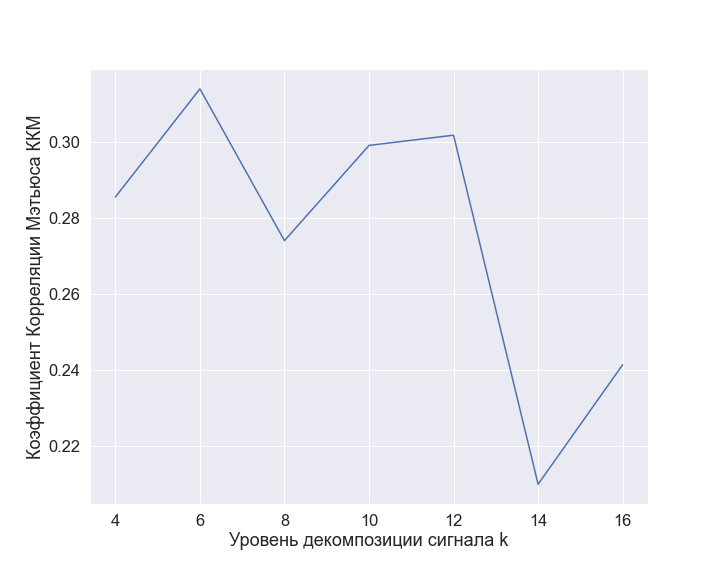
\includegraphics[scale = 0.55]{img/KKM(k).png}}
		\end{center}
		\caption{График зависимости\textit{Коэффициента Корреляции Мэтьюса ККМ} от уровня декомпозиции сигнала k.}
		\label{ris:auc(n_frame)}
	\end{figure}
	
	Из приведенного выше графика видно, что наибольшее значение параметр \textit{ММК} принимает при \textit{k} = 6.
	
	\subsection{Оценка качества модели классификации}
	
	Ниже приведены результаты применения описанных выше метрик на обученной модели классификации при выборе оптимальных параметров:
	
	\begin{center}
		\begin{longtable}[h!]{|p{0.3\linewidth}|p{0.3\linewidth}|p{0.3\linewidth}|}
			\hline
			{} & {precision} & {recall}\\
			\hline
			{positive} & {0.72} & {0.56}\\
			\hline
			{negative} & {0.63} & {0.77}\\
			\hline
			\caption{Точность (precision) и полнота (recall) предсказания модели.}
		\end{longtable}
	\end{center}

	Коэффициент Корреляции Мэтьюса (ККМ) равен 0.33.

	\begin{figure}[h!]
		\begin{center}
			{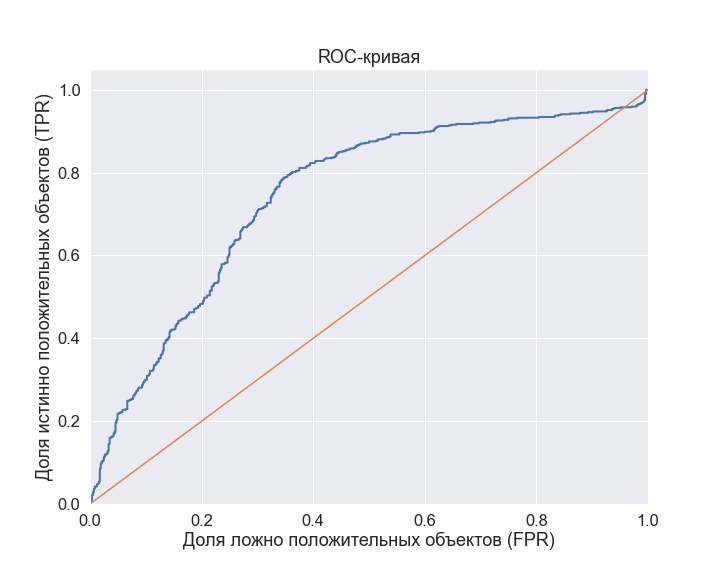
\includegraphics[scale = 0.55]{img/roc_curve.png}}
		\end{center}
		\caption{ROC-кривая.}
		\label{ris:roc_curve}
	\end{figure}

	При этом \textit{AUC} = 0.7325.
	
	В литературе \cite{auc} приводится следующая экспертная шкала для значений \textit{AUC}, по которой можно судить о качестве модели:
	
	\begin{center}
		\begin{longtable}[h!]{|p{0.3\linewidth}|p{0.3\linewidth}|}
			\hline
			{Интервал AUC} & {Качество модели}\\
			\hline
			{0.9-1.0} & {отличное}\\
			\hline
			{0.8-0.9} & {очень хорошее}\\
			\hline
			{0.7-0.8} & {хорошее}\\
			\hline
			{0.6-0.7} & {среднее}\\
			\hline
			{0.5-0.6} & {удовлетворительное}\\
			\hline
			\caption{Экспертная шкала значений AUC.}
		\end{longtable}
	\end{center}

	Откуда следует, что полученная модель имеет хорошее качество предсказания.
	
	\subsection{Выводы}
	
	В результате проведения исследовательской работы над разработанным методом были выполнены следующие задачи:
	
	\begin{itemize}
		\item были сформированы обучающие и тестовые выборки данных для обучения модели классификации обнаружения межфонемных переходов;
		\item были рассмотрены основные метрики оценки качества модели классификации применительно к данной задаче, а именно, к задаче с несбалансированными классами;
		\item был произведен поиск оптимальных гиперпараметров метода при помощи Коэффициента корреляции Мэтьюса (ККМ);
		\item была произведена оценка качества модели на оптимальных гиперпараметрах при помощи рассмотренных метрик.
	\end{itemize}

	Таким образом, полученная модель имеет хорошее качество предсказания, что означает, что разработанный метод может быть применим для решения задачи сегментации речевого сигнала.
	
	Такое относительно невысокое качество распознавания обусловлено малым размером обучающей выборки и сильной погрешностью измерений при разметке сформированных данных. Это связано с субъективностью человеческого слухового восприятия - все звуки размечались вручную разными людьми в результате чего возникла большая погрешность измерений.
	
	\pagebreak
	
	\section*{ЗАКЛЮЧЕНИЕ}
	\addcontentsline{toc}{section}{ЗАКЛЮЧЕНИЕ}
	
	В результате выполнения выпускной квалификационной работы были \linebreak успешно достигнуты все поставленные задачи:
	
	\begin{itemize}
		\item проанализирована предметная область:
		\begin{itemize}
			\item описаны основные этапы распознавания речевого сигнала;
			\item обоснована актуальность задачи сегментации речевого сигнала;
			\item проведен анализ существующих решений сегментации речевого сигнала.
		\end{itemize}
		\item проведен анализ существующих методов выделения признаков речевого сигнала и алгоритмов классификации;
		\item выбраны методы наиболее оптимальные для поставленной цели;
		\item на их основе спроектирован метод выделения звуков естественного языка в звучащей речи и разработан алгоритм, реализующий данный метод;
		\item спроектирована систему для проверки работоспособности метода;
		\item сформирована выборка для проведения эксперимента;
		\item проведено исследование разработанного метода на данной выборке;
	\end{itemize}

	Проведя исследование разработанного метода, выяснилось, что разработанный метод может быть применим для решения задачи сегментации речевого сигнала. Однако, реализованная модель имеет относительно невысокое качество предсказания, что обусловлено малым размером обучающей выборки и сильной погрешностью измерений при разметке сформированных данных. 
	
	Это связано с субъективностью человеческого слухового восприятия - все звуки размечались вручную разными людьми в результате чего возникла большая погрешность измерений.
	
	Можно обозначить следующие пути развития данной работы:
	
	\begin{itemize}
		\item подготовка большего количества обучающей выборки, имеющей меньшую погрешность измерений для повышения точности метода;
		\item применение альтернативных алгоритмов классификации, позволяющими повысить качество распознавания с применением большего количества данных.
	\end{itemize}
	
	\pagebreak
	
	\addcontentsline{toc}{section}{СПИСОК ИСПОЛЬЗОВАННЫХ ИСТОЧНИКОВ}
	
	\begin{thebibliography}{}
		\bibitem{ling_elem}
		Аграновский А.В., Леднов Д.А., Телеснин Б.А. Сегментация речи (математическая модель) // Информационные технологии. 1998. № 9. C. 24-28
		\bibitem{speech_phone_machines}
		Казачкин, А. Е. Методы распознавания речи, современные речевые технологии [Электронный ресурс]. - Режим доступа: 
		https://moluch.ru/archive/277/62675/, свободный - (17.03.2021)
		\bibitem{speech_people}
		Шпаков, Д. В. Распознавание голоса в сфере информационных технологий [Электронный ресурс]. - Режим доступа: https://moluch.ru/archive/163/45163/, свободный - (17.03.2021)
		\bibitem{speech_classification}
		Федосин С.А., Еремин А. Ю. Классификация систем распознавания речи. [Электронный ресурс]. - Режим доступа:
		http://fetmag.mrsu.ru/2010-2/pdf/SpeechRecognition.pdf, свободный - (19.04.2021)
		\bibitem{speech_modules}
		Тампель И.Б, Карпов А.А. Автоматическое распознавание речи. — СПб. : Университет ИТМО, 2016. — С. 113. [Электронный ресурс]. - Режим доступа: https://books.ifmo.ru/file/pdf/1921.pdf, свободный - (19.04.2021)
		\bibitem{rem}
		Рамишвили Г. С. Автоматическое опознавание говорящего по голосу. М. : Радио и
		связь, 1981. 224 с
		\bibitem{vevlet_1}
		О.А. Вишнякова, Д.Н. Лавров АВТОМАТИЧЕСКАЯ СЕГМЕНТАЦИЯ РЕЧЕВОГО СИГНАЛА НА БАЗЕ ДИСКРЕТНОГО ВЕЙВЛЕТ-ПРЕОБРАЗОВАНИЯ [Электронный ресурс]. - Режим доступа: http://msm.omsu.ru/jrns/jrn23/VishnyakovaLavrov.pdf, свободный - (22.04.2021)
		\bibitem{vevlet_2}
		Т. Ермоленко, В. Шевчук АЛГОРИТМЫ СЕГМЕНТАЦИИ С ПРИМЕНЕНИЕМ
		БЫСТРОГО ВЕЙВЛЕТ-ПРЕОБРАЗОВАНИЯ [Электронный ресурс]. - Режим доступа: http://www.dialog-21.ru/media/2715/ermolenko.pdf, свободный - (22.04.2021)
		\bibitem{hilbert_huang}
		О.А. Вишнякова, Д.Н. Лавров ПРИМЕНЕНИЕ ПРЕОБРАЗОВАНИЯ
		ГИЛЬБЕРТА-ХУАНГА К ЗАДАЧЕ СЕГМЕНТАЦИИ РЕЧИ [Электронный ресурс]. - Режим доступа: http://msm.omsu.ru/jrns/jrn24/Vishnakova\_n24\_2011.pdf, свободный - (10.05.2021)
		\bibitem{magistr}
		И.В. Дашкевич. МАГИСТЕРСКАЯ ДИССЕРТАЦИЯ Модуль голосовой идентификации диктора [Электронный ресурс]. - Режим доступа: http://elib.sfu-kras.ru/bitstream/handle/2311/74791/diplom\_magistratura.pdf?sequence=1, свободный - (23.04.2021)
		\bibitem{wavelet_neuron}
		Музычук, Д. С. Использование преобразования Гильберта-Хуанга для формирования моделей фонем русского языка в задаче распознавания речи [Электронный ресурс]. - Режим доступа: https://moluch.ru/archive/53/7041/, свободный - (15.05.2021).
		\bibitem{furie_from_wavelet_neuron}
		Давыдов А. В. Цифровая обработка сигналов: Тематические лекции. — Екатеринбург: УГГУ, ИГиГ, ГИН, Фонд электронных документов, 2005.
		\bibitem{disertation}
		Томчук Кирилл Константинович, Сегментация речевых сигналов
		для задач автоматической обработки речи [Электронный ресурс]. - Режим доступа: https://fs.guap.ru/dissov/tomchuk\_kk/full.pdf, свободный - (10.05.2021)
		\bibitem{classification_methods}
		Т.В. Батура, МЕТОДЫ АВТОМАТИЧЕСКОЙ КЛАССИФИКАЦИИ ТЕКСТОВ [Электронный ресурс]. - Режим доступа: https://www.researchgate.net/publication/315328102\_Metody\_avtomaticeskoj\_
		
		klassifikacii\_tekstov, свободный - (11.05.2021)
		\bibitem{svm}
		К.В. Воронцов Лекции по методу опорных векторов [Электронный ресурс]. - Режим доступа: http://www.ccas.ru/voron/download/SVM.pdf, свободный - (11.05.2021)
		\bibitem{oszilograph}
		Осциллографирование электрических сигналов цифровым осциллографом [Электронный ресурс]. - Режим доступа: https://portal.tpu.ru/SHARED/k/KOZHEMYAK/Teaching/Tab1/Electronics/
		
		Lab\_1\_Digital\_oscilloscope\_2018.pdf, свободный - (10.05.2021)
		\bibitem{python}
		Python documentation [Электронный ресурс]. - Режим доступа:
		https://www.python.org/doc/, свободный - (11.05.2021)
		\bibitem{pycharm}
		Pycharm documentation [Электронный ресурс]. - Режим доступа:
		https://www.jetbrains.com/help/pycharm/inline-documentation.html, свободный - (11.05.2021)
		\bibitem{librosa}
		Librosa documentation [Электронный ресурс]. - Режим доступа:
		https://librosa.org/doc/latest/index.html, свободный - (11.05.2021)
		\bibitem{pywt}
		PyWavelets documentation [Электронный ресурс]. - Режим доступа:
		https://pywavelets.readthedocs.io/\_/downloads/en/v1.0.0/pdf/, свободный - (11.05.2021)
		\bibitem{scikit-learn}
		Scikit-learn documentation [Электронный ресурс]. - Режим доступа:
		https://www.sklearn.org/documentation.html, свободный - (11.05.2021)
		\bibitem{pandas}
		Pandas documentation [Электронный ресурс]. - Режим доступа:
		https://pandas.pydata.org/pandas-docs/stable/index.html, свободный - (11.05.2021)
		\bibitem{matplotlib}
		Matplotlib documentation [Электронный ресурс]. - Режим доступа:
		https://matplotlib.org/, свободный - (11.05.2021)
		\bibitem{numpy}
		NumPy documentation [Электронный ресурс]. - Режим доступа:
		https://numpy.org/doc/, свободный - (11.05.2021)
		\bibitem{pyqt5}
		PyQt5 documentation [Электронный ресурс]. - Режим доступа:
		https://doc.qt.io/qtforpython/, свободный - (11.05.2021)
		\bibitem{cross-val}
		Кросс-валидация [Электронный ресурс]. - Режим доступа:
		http://datascientist.one/cross-validation/, свободный - (06.04.2021)
		\bibitem{auc}
		Zweig, Mark H.; Campbell, Gregory. Receiver-operating characteristic (ROC) plots: a fundamental evaluation tool in clinical medicine. Clinical
		Chemistry. Нью-Йорк: Изд-во Oxford, 577 с.
	\end{thebibliography}

	\label{last}
	\pagebreak
	
	\section*{ПРИЛОЖЕНИЕ A}
	\addcontentsline{toc}{section}{ПРИЛОЖЕНИЕ A}
	
	Ниже приведены листинги разработанного ПО.

	{\bf MainView}
	\lstinputlisting[lastline=38]{prog/view/main_view/main_window.py}
	\newpage
	{\bf MainView}
	\lstinputlisting[firstline=39, lastline=78]{prog/view/main_view/main_window.py}
	\newpage
	{\bf ResultView}
	\lstinputlisting{prog/view/result_view/result_window.py}
	\newpage
	{\bf TeachModelView}
	\lstinputlisting[lastline=40]{prog/view/teach_model_view/teach_model_window.py}
	\newpage
	{\bf TeachModelView}
	\lstinputlisting[firstline=41]{prog/view/teach_model_view/teach_model_window.py}
	
	{\bf MainController}
	\lstinputlisting[lastline=10]{prog/controller/main_controller/main_controller.py}
	\newpage
	{\bf MainController}
	\lstinputlisting[firstline=11]{prog/controller/main_controller/main_controller.py}
	\newpage
	{\bf ResultController}
	\lstinputlisting{prog/controller/result_controller/result_controller.py}
	{\bf TeachModelController}
	\lstinputlisting[lastline=24]{prog/controller/teach_model_controller/teach_model_controller.py}

	\newpage
	
	{\bf ClassificationModule}
	\lstinputlisting[lastline=39]{prog/model/classification_module/classification_module.py}
	\newpage
	{\bf ClassificationModule}
	\lstinputlisting[firstline=40]{prog/model/classification_module/classification_module.py}
	\newpage
	{\bf DataPreprocessingModule}
	\lstinputlisting[lastline=36]{prog/model/data_preprocessing_module/data_preprocessing_module.py}
	\newpage
	{\bf DataPreprocessingModule}
	\lstinputlisting[firstline=37, lastline=76]{prog/model/data_preprocessing_module/data_preprocessing_module.py}
	\newpage
	{\bf FeatureExtractionModule}
	\lstinputlisting[lastline=44]{prog/model/feature_extraction_module/feature_extraction_module.py}
	\newpage
	{\bf FeatureExtractionModule}
	\lstinputlisting[firstline=44]{prog/model/feature_extraction_module/feature_extraction_module.py}
	\newpage
	{\bf GraphModule}
	\lstinputlisting{prog/model/graph_module/graph_module.py}
	{\bf LoadDataModule}
	\lstinputlisting[lastline=25]{prog/model/load_data_module/load_data_module.py}
	\newpage
	{\bf LoadDataModule}
	\lstinputlisting[firstline=26, lastline=63]{prog/model/load_data_module/load_data_module.py}
	\newpage
	{\bf LoadDataModule}
	\lstinputlisting[firstline=64]{prog/model/load_data_module/load_data_module.py}
	{\bf SoundsExtractionModule}
	\lstinputlisting[lastline=23]{prog/model/sounds_extraction_module/sounds_extraction_module.py}
	\newpage
	{\bf SoundsExtractionModule}
	\lstinputlisting[firstline=24,lastline=62]{prog/model/sounds_extraction_module/sounds_extraction_module.py}
	\newpage
	{\bf SoundsExtractionModule}
	\lstinputlisting[firstline=63, lastline=100]{prog/model/sounds_extraction_module/sounds_extraction_module.py}
	\newpage
	{\bf Parameters}
	\lstinputlisting{prog/model/data.py}
	\lstinputlisting{prog/model/params/audio_params.py}
	\lstinputlisting{prog/model/params/classification_params.py}
	\newpage
	{\bf Parameters}
	\lstinputlisting{prog/model/params/markups_params.py}
	
	\pagebreak
	
\end{document}